\documentclass[pra,
aps,
twocolumn,
superscriptaddress,
groupedaddress,
nofootinbib,
reprint
]{revtex4-1}

% PACKAGES
\usepackage{amsmath,amsfonts, amssymb, amsthm}
\usepackage{bm, bbm, physics, mathtools}
\usepackage{graphicx, subfigure}
\usepackage{xcolor, enumerate}
\usepackage{xifthen, hyperref}
\usepackage[capitalise]{cleveref}

\hypersetup{
	colorlinks=true,  
	linkcolor=blue,   
	citecolor=blue,   
	urlcolor=blue     
}

\newcommand{\crefrangeconjunction}{--}
\creflabelformat{figure}{(#2#1#3)}

% COMMENT NOTATION
\newcommand{\nick}[1]{{\color{red}#1}}
\newcommand{\ddd}[1]{\textcolor{blue}{#1}}

% ENVIRONMENTS
\newtheorem{theorem}{Theorem}
\newtheorem{proposition}[theorem]{Proposition}
\newtheorem{lemma}[theorem]{Lemma}
\newtheorem{definition}[theorem]{Definition}

% REFERENCES
\iffalse
\renewcommand{\eqref}[1]{Eq.~(\ref{#1})}
\newcommand{\figref}[1]{Fig.~(\ref{#1})}
\newcommand{\tabref}[1]{Tab.~(\ref{#1})}
\newcommand{\secref}[1]{Section~(\ref{#1})}
\newcommand{\appref}[1]{Appendix~(\ref{#1})}
\newcommand{\defref}[1]{Definition~\ref{#1}}
\newcommand{\lemref}[1]{Lemma~\ref{#1}}
\newcommand{\thmref}[1]{Theorem~\ref{#1}}
\fi

% SYMBOL DEFINITIONS
\renewcommand{\cal}[1]{\mathcal{#1}}

\newcommand{\reals}{\mathbb{R}}
\newcommand{\id}{\mathbbm{1}}
\newcommand{\idc}{1_{\rm{C}}}
\newcommand{\supf}{\mathfrak{c}}
\renewcommand{\tr}{{\rm{tr}}}
\renewcommand{\det}{{\rm{det}}}
\newcommand{\floor}[1]{\left\lfloor #1 \right\rfloor}
\newcommand{\ent}[2]{S\left( #1 \middle\vert\middle\vert #2 \right)}
\newcommand{\ents}{{\ent{\frac{m}{n}}{p}}}

\def\dummy{\ell}
\def\NN{n}
\def\mmf{i}
\def\nnf{n}
\def\mlt{m}
\def\ii{i}
\def\jj{j}
\def\kk{k}
\def\II{I}
\def\nn{n}
\def\tt{n'}
\def\mm{a}
\def\wp{u}
\def\wn{v}

\newcommand{\too}[1]{^{\otimes #1}}
\newcommand{\noisys}{\rho_{\rm{S}}}
\newcommand{\noisysn}{\rho_{\rm{S}}(\epsilon)^{\otimes \nn}}
\newcommand{\noisysN}{\rho_{\rm{S}}(\epsilon)^{\otimes \NN}}

\newcommand{\spanv}[1]{
    {{\rm{span}}\left\{#1\right\}}
}
\newcommand{\conv}[1]{
    {{\rm{conv}}#1}
}
\newcommand{\orb}[1]{
    {{\rm{orb}}(#1)}
}
\newcommand{\sn}[1]{
    {{\rm{sn}}\left(#1\right)}
}
\newcommand{\mana}[1]{
    {{\rm{mana}}\left(#1\right)}
}
\newcommand{\lc}[2]{
	{{\rm{L}}_{#1|#2}}
}

\newcommand{\bmx}{\bm{x}}
\newcommand{\bmy}{\bm{y}}
\newcommand{\bmz}{\bm{z}}
\newcommand{\bmu}{\bm{u}}
\newcommand{\bmw}{\bm{w}}
\newcommand{\bmo}{\bm{0}}
\newcommand{\bmd}{\bm{d}}
\newcommand{\bma}{\bm{a}}
\newcommand{\bmxi}{\bm{\xi}}
\newcommand{\bmg}{\bm{g}}

\newcommand{\zd}[1][]{
    \ifthenelse{\isempty{#1}}{
    {\mathbb{Z}_d} }{
    {\mathbb{Z}_{#1}}}
}
\newcommand{\hd}[1][]{
    \ifthenelse{\isempty{#1}}{
    {\cal{H}_d} }{
    {\cal{H}_{#1}}}
}
\newcommand{\pd}[1][]{
    \ifthenelse{\isempty{#1}}{
    {\cal{P}_d} }{
    {\cal{P}_{#1}}}
}
\newcommand{\cd}[1][]{
    \ifthenelse{\isempty{#1}}{
    {\cal{C}_d} }{
    {\cal{C}_{#1}}}
}
\newcommand{\spd}[1][]{
    \ifthenelse{\isempty{#1}}{
    {{\rm{Sp}}(2, \zd)} }{
    {{\rm{Sp}}(2, \zd[#1])}}
}
\newcommand{\gp}[1][]{
    \ifthenelse{\isempty{#1}}{
    {\rm{GP}_d} }{
    {\rm{GP}_{#1}}}
}
\newcommand{\stoch}[1][]{
    \ifthenelse{\isempty{#1}}{
    {{\rm{S}}_d(\bmd)} }{
    {{\rm{S}}_d(#1)}}
}
\newcommand{\stochw}[1][]{
    \ifthenelse{\isempty{#1}}{
    {{\rm{S}}_{d^2}(\W{\sigma})} }{
    {{\rm{S}}_{d^2}(#1)}}
}
\makeatletter
\def\W{\@ifnextchar[{\@with}{\@without}}
\def\@with[#1]#2{ 
    {{\rm{W}}_{#2}\left(#1\right)} }
\def\@without#1{ 
    {{\rm{W}}_{#1}} }
\makeatother

\newcommand{\T}{\cal{T}}
\newcommand{\Z}{\cal{Z}}

\newcommand{\C}{\cal{C}}
\newcommand{\E}{\cal{E}}
\newcommand{\J}{\cal{J}}
\newcommand{\R}{\cal{R}}
\newcommand{\D}{\cal{D}}
\newcommand{\F}{\cal{F}}
\renewcommand{\O}{\cal{O}}
\newcommand{\M}{\cal{M}}

\newcommand{\Fmax}{\F_{\rm{max}}}
\newcommand{\Omax}{\O_{\rm{}max}}
\newcommand{\Rmax}{\R_{\rm{}max}}
\newcommand{\Pis}{\Pi_{\rm{s}}}
\newcommand{\Pio}{\Pi_{\rm{o}}}

\newcommand{\cptp}{{\rm{CPTP}}}
\newcommand{\cpos}{{\rm{CP}}}
\newcommand{\so}{{\rm{SO}}}
\newcommand{\stab}{{\rm{STAB}}}
\newcommand{\spo}{{\rm{SPO}}}
\newcommand{\cspo}{{\rm{CSPO}}}
\newcommand{\rcu}{{\rm{RCU}}}
\newcommand{\tho}{{\rm{TO}}}
\newcommand{\cpwp}{{\rm{CPWPO}}}
\newcommand{\ru}{{\rm{RU}}}


\begin{document}
% - vs -- (n-copy, sigma--fragment etc.)
% Distillation rate vs bound
% Sec: Appendix D
% Sec: Intro
% Sec: General resources
% Sec: Lower bounds
% Sec: Abstract
% Plot consistency (esp. figs 3,4,5,6)
% Spacing

\begin{abstract}
\ddd{[To be sharpened]} Magic states are key ingredients in schemes to realise universal fault-tolerant quantum computation.
Theories of magic states attempt to quantify this computational element via monotones and determine how these states may be efficiently transformed into useful forms. Here we introduce the concept of `fragments', which generalise the concept of magic monotones and has a natural thermodynamic structure based on majorisation. From this perspective magic can be viewed as a form of free energy within each fragment and is constrained by relative majorisation relations but now on quasi-probability distributions. Notably this approach allows us to incorporate actual physical constraints, for example noise models with particular bias or temperature-dependent features, and study how these constrain general magic distillation protocols. In this context we present general temperature-dependent bounds on distillation rates that any theory of magic must respect. Significantly, this analysis also presents a thermodynamic context which cannot be analysed via traditional methods based on thermodynamic entropies, due to the presence of negativity, and raises novel questions in the context of statistical mechanics.
\end{abstract}

\preprint{APS/123-QED}

\title{Thermodynamic fragments for magic states in quantum computation}

\author{Nikolaos Koukoulekidis}
	\email{nk2314@imperial.ac.uk}
	\affiliation{Department of Physics, Imperial College London, London SW7 2AZ, UK}
\author{David Jennings}
	\affiliation{School of Physics and Astronomy, University of Leeds, Leeds, LS2 9JT, UK}
	\affiliation{Department of Physics, Imperial College London, London SW7 2AZ, UK}

\date{\today}
\maketitle

%%%%%%%%%%%%%%%%%%%%%%%%%%%%%%%%%%%%%%%%

\section{Introduction and background}
\label{sec:intro_prev}

\subsection{Introduction}
\label{sec:intro}

Magic states are necessary for achieving universal quantum computation within fault-tolerant schemes~\cite{cit:veitch, cit:mari, cit:gottesman, cit:bravyi, cit:knill, Campbell_2011}.
Identifying magic as a resource for quantum universality has led to several theories which try to provide a framework for its quantification and manipulation \cite{cit:veitch2, cit:howard, Wang_2019, Seddon_2021}.
The main question that such a theory attempts to answer is:
\begin{center}
    \emph{Given two magic states $\rho$ and $\rho'$ is there a free operation that can convert $\rho$ to $\rho'$?}
\end{center}

We are interested in all resource theories of magic $\R = (\F, \O)$ in which free operations cannot generate any amount of resource. 
Further denote by $\D$ the set of states considered under the theory, that is the union of free and resource states.
The structure of such theory is described by a partial order, hereinafter called a \emph{pre-order}, $\prec_{\R}$ between states.
We write $\rho' \prec_{\R} \rho$ iff there exists $\E \in \O$ such that $\E(\rho) = \rho'$.
Naturally, states may be incomparable under the given theory, meaning that there exists no free operation that converts one to the other.
We further call $\R' = (\F', \O')$ a \emph{subtheory} of $\R$ iff $\F' \subseteq \F$ and $\O' \subseteq \O$. 
The above notation will be used for general resource theories as well.

Formally, the no resource generation condition on the theories translates into two assumptions:
\begin{enumerate}[I]
    \item Free operations send free states into free states, $\E: \F \mapsto \F$, for all $\E \in \O$;
    \item Resource theory $\R$ is a completely free state preserving theory, in the sense that for any $d$--dimensional ancilla system and all free operations $\E$, $(\id_d \otimes \E ) \sigma \in \F$ whenever $\sigma \in \F$.
\end{enumerate}
The first assumption simply states that resources cannot be generated for free and is a minimal requirement for a resource theory. 
An immediate consequence is that if statistical mixing is included in $\O$, then the resource theory is convex.

Monotones are often used to address the question of state convertibility, although such approaches are usually generic.

The monotonicity condition reflects the no resource generating property of free operations, so that monotones respect the pre-order $\prec_\R$ of the theory.
A monotone of any general resource theory is a projection of the theory onto the non-negative real numbers, collapsing the pre-order of the theory to the total order defined on the real line.
Our contribution is the introduction of a generalised notion of \emph{resource projection} which maps a general resource theory onto a subtheory which in principle still retains a partial structure (as opposed to the real line).
Applying this notion on existing magic theories highlights the hidden stochasticity that governs magic state conversions.
We show that a magic theory can be subdivided into \emph{fragments} \nick{FIX AND EXPAND}

\subsection{Previous work}
\label{sec:prev}

The stabiliser theory of magic comprises of the so-called ``stabiliser'' states ($\stab$) and operations ($\so$), while non-stabiliser (resource) states are called magic.
The stabiliser operations can be expressed in terms of a Stinespring dilation as 
\begin{equation}
    \E(\rho) = \tr_E [U(\rho \otimes \sigma_E)U^\dagger],
\end{equation} 
for an ancilla stabiliser state $\sigma_E$. 
The motivation of the theory stems from the fact that stabiliser operations are experimentally straightforward to implement and they can be used to detect and correct errors on the stabiliser states due to their construction \cite{cit:gottesman, cit:gottesman2, cit:gottesman1998}.
The Gottesman-Knill theorem however indicates that stabiliser operations need to be supplemented with magic states in order to achieve universality, justifying the term ``magic''.

Generalisations of the stabiliser theory appear in the literature intending to include broader classes of operations.
The class of stabiliser preserving operations ($\spo$) is defined as the set of $\cptp$ maps that send stabiliser states into stabiliser states~\cite{cit:ahmadi}.
An important subclass of $\spo$ is the set of completely stabiliser preserving operations ($\cspo$)~\cite{cit:seddon}, which intuitively cannot induce ``non-stabiliserness'' even when applied to only part of a quantum state, i.e. operations $\E$ such that $(\id_d \otimes \E ) \sigma \in \stab$ for all positive dimensions $d$ whenever $\sigma \in \stab$.

Even though non-stabiliserness is a necessary resource for universality, it has been proven insufficient for magic state distillation~\cite{cit:bravyi, cit:campbell}.
In fact, all states with non-negative Wigner distributions have been proven to be efficiently classically simulable in~\cite{cit:mari}, a result that serves as a generalization of the Gottesman-Knill theorem.
The Wigner distribution of a state in odd prime dimensions, formally defined in~\cref{sec:wigner}, arises as the unique quasi-probability representation of quantum theory that identifies non-contextuality exactly with the states that are efficiently classically simulable~\cite{Delfosse_2017, cit:howard2, cit:veitch2}.
In this framework, the stabiliser states are the only pure states represented with non-negative distributions~\cite{cit:gross3}. 
However, there exist mixed states with non-negative Wigner distributions that are not mixtures of stabiliser states~\cite{cit:gross}.
Therefore, stabiliser-preserving theories have been extended to a theory that preserves state ``Wigner positivity''~\cite{Wang_2019}.
Informally, it can be considered as the maximal theory of magic $\Rmax = (\Fmax, \Omax)$, where free states have non-negative Wigner distributions and free operations completely preserve this property.\\ 

\ddd{Things we MUST emphasize:
\begin{enumerate}
\item Perhaps a nice lead-in question: ``What happens if we view stabiliser states as thermodynamic equilibrium states and magic as a form of free energy?''
\item We have found a scenario in which it is impossible to describe a thermodynamic structure using any entropic approach!
\item We can tackle more `physicsy' questions like: how much magic can be distilled via available operations with some given fixed-point structure? 
\item This allows a diagnostic on the kind of operations needed to do good distillation. I.e. what fixed point structure should they have?
\item We go beyond the concept of monotones and replace a monotone with a $\sigma$--fragment.
\item We can get both upper and lower bounds on magic distillation.
\end{enumerate}
}
%%%%%%%%%%%%%%%%%%%%%%%%%%%%%%%%%%%%%%%%

\newpage
\section{Phase space representations of quantum states}
\label{sec:ps}

Central to our construction is the representation of any quantum state or quantum operation on a system of dimension $d$ in terms of quasi-probability representations on a discrete phase space \ddd{[CITE the review on quasi-reps]}. This construction is a discrete version of Wigner representations in quantum optics.

We consider a $d$--dimensional quantum system with Hilbert space $\H_d$, and let $\{ |0\>, |1\>, \dots , |d-1\>\}$ denote the standard computational basis, defined over $\mathbb{Z}_d = \{ 0, 1, \dots,d-1 \}$. On this space, generalised Pauli matrices $X, Z$ can be defined by their respective roles as shift and phase operators, which act on the basis states as follows,
\begin{align}
    X \ket{k} &= \ket{k + 1} \label{eq:xpauli}\\
	Z \ket{k} &= \omega^k \ket{k}. \label{eq:zpauli}
\end{align}
Here $\omega \coloneqq e^{2\pi i/d}$ is the $d$-th root of unity and addition is taken modulo $d$. From these we can construct a phase space $\cal{P}_d = \mathbb{Z}_d \times \mathbb{Z}_d$ that provides a complete representation of the quantum system. Given a point $\bmx \coloneqq (x, p)$ we define a displacement operator, 
\begin{equation}\label{eq:ddef}
    D_{\bmx} \coloneqq \tau^{x p} X^{x} Z^{p},\ 
\end{equation}
where a phase factor $\tau \coloneqq -\omega^{1/2}$ ensures unitarity. We assume going forward that $d$ is an odd prime, however the case $d=2$ can be also handled, but with some additional technical caveats \ddd{[CITE]}. For a composite system with composite dimension $d = d_1 \dots d_n$ we can decompose the Hilbert space as $\cal{H}_d = \cal{H}_{d_1} \otimes \dots \otimes \cal{H}_{d_n}$, and then define displacement operators as
\begin{equation}\label{eq:composited}
    D_{\bmx} \coloneqq D_{(x_1, p_1)} \otimes \dots \otimes D_{(x_n, p_n)},
\end{equation}
where now we have
\begin{align*}
	\bmx \coloneqq (x_1, p_1, x_2, p_2, \dots, x_n, p_n) \in \cal{P}_{d_1} \times \dots \times \cal{P}_{d_n} \eqqcolon  \cal{P}_d,
\end{align*}
to denote the phase space point for the composite system. For simplicity going forward we assume $n$ copies of a $d$--dimensional system $d_1=d_2 = \cdots = d$, and therefore, we have that $\x \in \mathbb{Z}_d^{2n}$.


The displacement operators form the Heisenberg-Weyl group~\cite{Folland_1989, Bengtsson_2006} under matrix multiplication modulo phases,
\begin{equation}\label{eq:gp}
    {\rm{HW}}_d^n \coloneqq \{ \tau^k D_{\bmx}: k \in \mathbb{Z}_d, \bmx \in \cal{P}_d^n\}.
\end{equation}
The Clifford operations $ \cal{C}_d^n $ are then defined as the set of unitaries that normalise the Heisenberg-Weyl group \ddd{[CITE]}. We may define the pure stabiliser states as those states obtained by acting on $|0\>$ with Clifford unitaries. Finally, we define $\stab$ as the convex hull of all pure stabiliser states, namely all probabilistic mixtures of states of the form $U|0\>\<0|U^\dagger$ where $U$ is some Clifford unitary. 

\subsection{Wigner representations for quantum states and quantum operations}\label{sec:wigner}

In order to provide a complete decomposition of arbitrary quantum states and quantum operations we now define a complete basis of hermitian observables that behaves naturally under the action of the Clifford group. To every point $\x \in \P_d$ we define the phase-point operator $A_{\x}$ given by
\begin{align}
	A_{\bmx} \coloneqq \frac{1}{d} \sum_{\bmz \in \cal{P}_d} \omega^{\eta(\bmx, \bmz)} D_{\bmz}, \label{eq:ax}
\end{align}
where $\eta(\bmx, \bmz)$ is the symplectic inner product between any two points $\x,\z \in \P_d$, and is given explicitly by
\begin{equation}
	\eta(\bmx, \bmz) \coloneqq \bmz^T \begin{pmatrix}
		0  & \id \\ %\mathbbm{O}_n  & \id_n \\
		-\id & 0 \\ %-\id_n & \mathbbm{O}_n \\
	\end{pmatrix} \bmx,
\end{equation}
where $0, \id$ denote the $n\times n$ zero and identity matrices.

The phase-point operators form an orthogonal (with respect to the Hilbert-Schmidt inner product) operator basis as shown in~\cref{app:wigner}.
Therefore, any quantum state $\rho \in \cal{B}(\cal{H}_d)$ can be expressed as a linear combination of them,
\begin{equation}
    \rho = \sum_{\bmz \in \cal{P}_d} \W[\bmz]{\rho} A_{\bmz},
\end{equation}
where the coefficient vector $\W{\rho}$ is the Wigner distribution of state $\rho$,
\begin{equation}\label{eq:wstate}
    \W[\bmx]{\rho} \coloneqq \frac{1}{d}\tr[A_{\bmx} \rho].
\end{equation}


For any quantum state $\rho$, the Wigner distribution $W_\rho(\bmx)$ is readily seen to be a $d^2$-dimensional quasi-probability distribution over $\cal{P}_d$ (see~\cref{app:wigner} for details). More precisely, $W_\rho(\x)$ is a real-valued function on $\P_d$ with the property that $\sum_{\x} W_\rho(x) = 1$.  In~\cref{fig:wstate_examples}, we show Wigner distributions of different types of qutrit states.

\begin{figure}%
    \centering
    \subfigure[][]{%
    \label{fig:maxmix}%
    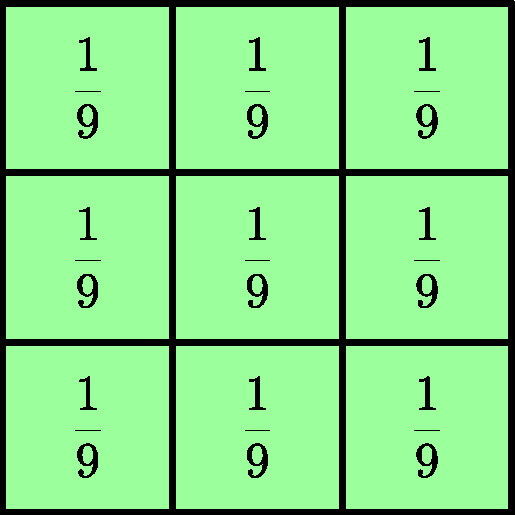
\includegraphics[height=2cm]{figs/maxmixed.pdf}
    %\caption{Maximally mixed state $\frac{1}{3}\id$}%
    }\hspace{8pt}%
    \subfigure[][]{%
    \label{fig:zero}%
    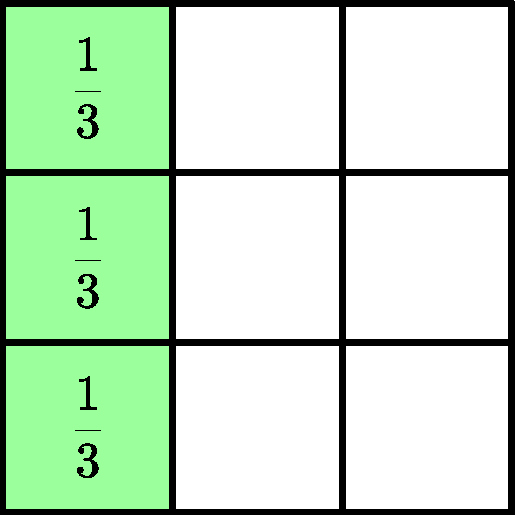
\includegraphics[height=2cm]{figs/zerostate.pdf}
    %\caption{Zero state $\ketbra{0}{0}$}%
    }\\
    \subfigure[][]{%
    \label{fig:bound}%
    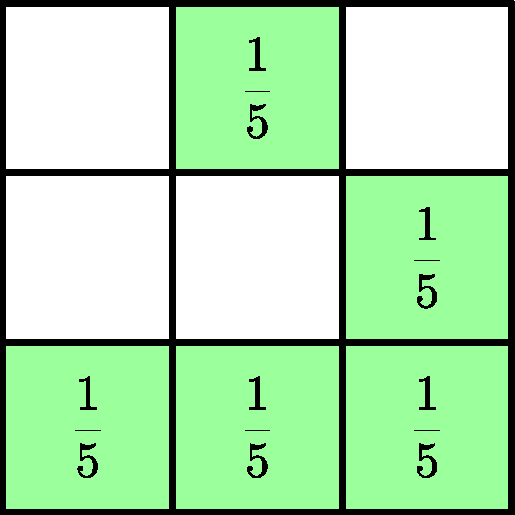
\includegraphics[height=2cm]{figs/boundstate.pdf}
    %\caption{Bound state}%
    }\hspace{8pt}%
    \subfigure[][]{%
    \label{fig:strange}%
    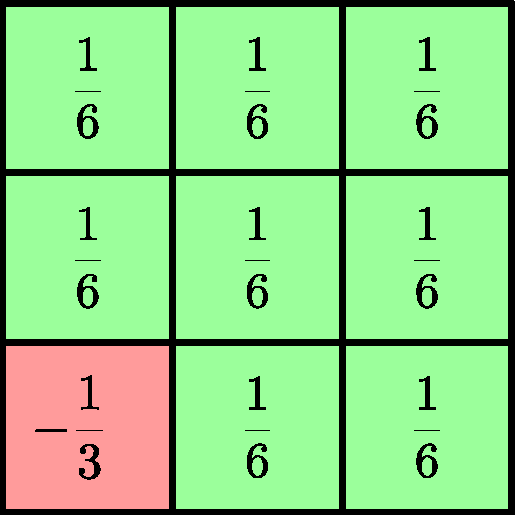
\includegraphics[height=2cm]{figs/strangestate.pdf}
    %\caption{Strange state $\ketbra{S}{S}$}%
    }
    \caption{\textbf{Qutrit Wigner distributions of varying magic.} 
    \subref{fig:maxmix} Maximally mixed state $\frac{1}{3}\id$; \subref{fig:zero} Stabilizer zero state $\ketbra{0}{0}$; \subref{fig:bound} A non-stabiliser Wigner-positive state; \subref{fig:strange} Magic Strange state $\ket{{\rm{S}}} = \frac{1}{\sqrt{2}}(\ket{1} - \ket{2})$, coined in~\cite{cit:veitch2}.
    }%
    \label{fig:wstate_examples}
\end{figure}


\subsection{Magic theories for quantum computation}
\label{sec:mono}

The state-injection model for quantum computation \ddd{[CITE]} is a key avenue to realising a full-scale, fault-tolerant quantum computer. Within the approach Clifford unitaries can be done in a robust, fault-tolerant way. However, due to the Eastin-Knill theorem \ddd{[CITE]}, it is impossible to have a universal set of transversal gates and so while Clifford unitaries can be realised transversally one must find ways around the Eastin-Knill restriction. The state-injection approach supplements the Clifford gates with noisy quantum states, called `magic states', that are outside the set of stabliser states and, when incorporated into Clifford circuits, provides universality. The obstacle to this is that the states are invariably noisy and so protocols must be employed so as to purify many copies of the magic states and improve the overall performance of the induced quantum gates. A central question is then: given a number $n$ of noisy magic states how many purified magic states can we obtain within the fault-tolerant set of quantum operations?

To address such questions both concrete distillation protocols have been developed, and there has been analysis of bounds of distillation rates within natural theoretical frameworks. These frameworks provide theories of magic in which one views magic states as ``resource'' states with respect to a natural class of quantum operations that are consider cheap, or ``free'' \ddd{[CITE Gour resource review]}. One very natural class of free operations considered are those obtained from Clifford operations, measurements and the ability to discard quantum systems. However there are several other candidate frameworks. 

For any theory of magic a natural route to bounding the distillation rates obtainable is through the concept of a \emph{magic monotone}. A magic monotone is a real-valued function of any quantum state $\M(\rho)$ that is monotonically non-increasing under the free operations of the magic theory. More precisely $\M(\sigma) \le \M(\rho)$ whenever it is possible to convert $\rho$ into $\sigma$ using at least one of the free operations available (e.g. Clifford operations).

One of the most fundamental and commonly used magic monotones is the \emph{mana} of a state~\cite{cit:veitch2}, defined as
\begin{equation}
    \mana{\rho} \coloneqq \ln{(2\hspace{1pt}\sn{\rho}+1)},
\end{equation}
where the \emph{sum-negativity}~\cite{cit:veitch2} is the sum of the negative components in $\W{\rho}$,
\begin{equation}
    \sn{\rho} \coloneqq \sum\limits_{\bmx: \W[\bmx]{\rho} < 0} \abs{\W[\bmx]{\rho}}.
\end{equation}

Mana is an additive\footnote{It satisfies the condition $\mana{\rho_1 \otimes \rho_2} = \mana{\rho_1} + \mana{\rho_2}$ which is practical in distillation settings.} magic monotone, so it provides an analytical, necessary condition for many-copy magic state interconvertibility.

A range of other monotones have been developed in the literature\cite{Wang_2018} \ddd{[CITE MORE]}, and each provides a means to upper bound distillation rates within a particular theory of magic. In this work we shall consider a broad framework for magic, with conditions that any theory of magic should satisfy. However, in contrast to prior works we shall not construct magic monotones, but instead develop a generalisation to resource monotones. The approach we take will also allow us to address how distillation rates are constrained by physical properties -- such as a system having biased-noise, some equilibrium structure or operations that manifest invariances, such as axial symmetry around the qubit $Z$-axis.



%%%%%%%%%%%%%%%%%%%%%%%%%%%%%%%%%%%%%%%%

\section{Stochastic structure of magic theories}
\label{sec:struc}

We also have Wigner representations for general quantum channels. We may exploit the channel-state duality and use the normalised Choi-Jamio\l{}kowski state 
\begin{equation}\label{eq:cj}
  \J(\E) \coloneqq \frac{1}{d_A}(\id \otimes \E) \sum_{i,j} \ket{ii}\bra{jj}
\end{equation}
to extend the definition of the Wigner distribution to a quantum channel $\E: \B(\H_A) \rightarrow \B(\H_B)$, via the expression
\begin{align}\label{eq:woperation}
    \W[\bmy|\bmx]{\E} 
    &\coloneqq d_A^2 \W[\bm{\bar x} \oplus \bmy]{\J(\E)} \\
    &= \frac{1}{d_B} \tr_B[A_{\bmy} \E(A_{\bmx})],
\end{align}
where $\bm{\bar x} \coloneqq (x, -p)$.

The specific form of~\cref{eq:woperation} is chosen so that Wigner distributions of operations act as transition matrices for Wigner distributions of states, $\W{\E(\rho)} = \W{\E}\W{\rho}$.
In particular, $\cptp$ operations that map between density operators of equal dimensions and have non-negative Wigner distributions correspond to stochastic matrices, as shown in~\cref{app:wigner}
\subsection{Magic fragments}\label{sec:magfrag}

Equipped with the definitions of the Wigner distribution in odd prime dimensions, we can formally recast the maximal magic theory $\Rmax$ into a stochasticity setting.
The free states correspond to proper probability distributions 
\begin{equation}
    \Fmax \coloneqq \{ \rho: \W[\bmx]{\rho} \geq 0 \text{ for all } \bmx \in \cal{P}_d\}
\end{equation}

The free operations should send the set of free states $\Fmax$ into itself and completely preserve the non-negativity of the states, in the sense that $\E \in \Omax$ iff $(\id_d \otimes \E ) \sigma \in \stab$ for all odd prime dimensions $d$ whenever $\sigma \in \Fmax$.
It is shown by Wang \textit{et al.}~\cite{Wang_2019} that $\Omax$ coincides with the set of operations $\E$ with stochastic Wigner distributions, 
\begin{equation}
    \Omax = \{ \E: \W[\bmy|\bmx]{\E} \geq 0 \text{ for all } \bmx, \bmy \in \cal{P}_d\}.
\end{equation}

Every established magic theory $\R = (\F, \O)$ is a subtheory of $\Rmax$ in the sense that $\F \subseteq \Fmax$ and $\O \subseteq \Omax$, and as such it falls under this new stochasticity setting. 
For technical simplicity in what follows we assume that $\F$ is a closed set, and note that $\F_{\rm{ max}}$ is itself a closed set, since it is specified by a finite set of linear constraints of the form $\tr[ L\rho] \geq 0$ with operators $L \in \cal{B}(\cal{H})$ ensuring that the state is positive and Wigner-positive.


Given this context we now define the following key notion, that is central to our analysis.
\begin{definition}[\textbf{$\boldsymbol\sigma$--fragment}]\label{def:sigmafrag}
   Given a resource theory of magic $\R = (\F, \O)$, the \emph{$\sigma$--fragment of $\R$} is the resource theory $\R_\sigma = (\F_\sigma, \O_\sigma)$, where $\F_\sigma = \{\sigma\}$ and the free operations are restricted to the ones that leave $\sigma$ invariant,
    \begin{equation}
        \O_\sigma \coloneqq \{ \E \in \O: \E(\sigma) = \sigma \}.
    \end{equation}
\end{definition}

Note that $\F = \bigcup_{\sigma \in \F} \F_\sigma$ trivially.
With this basic notion defined, we now show that this union holds for free operations as well and therefore that any resource theory of magic can be faithfully subdivided into $\sigma$--fragments, in such a way that any problem of interconversion in the parent magic theory $\R$ can be analysed across the different fragments.

\begin{theorem}\label{thm:frag}
    Let $\R = (\F, \O)$ be a theory of magic.
    Every operation in $\O$ leaves at least one free state invariant,
  \begin{equation}
\O = \bigcup\limits_{\sigma \in \F} \O_\sigma.
\end{equation}
Therefore, $\rho \longrightarrow \tau$ in $\R$ if and only if $\rho \longrightarrow \tau$ in a $\sigma$--fragment of $\R$.
\end{theorem}
\begin{proof}
    Suppose $\E$ is in a $\sigma$--fragment $\O_\sigma$.
    Then it is also in $\O$, hence $\bigcup\limits_{\sigma \in \F} \O_\sigma \subseteq \O$. 
    
    Conversely, suppose $\E$ is in $\O$. 
    The free states are a closed set that is mapped one-to-one to a closed subset $\cal{S}$ of the $(d^2 - 1)$--dimensional probability simplex.
    $\cal{S}$ is convex, since any combination of free states is also free and the Wigner distribution is linear.
    Therefore, $\cal{S}$ is convex and compact as a closed convex subset of the bounded compact probability simplex.
    
    We can now view $\W{\E}$ as a stochastic, continuous mapping from $\cal{S}$ to itself, thus Brouwer's fixed point theorem~\cite{cit:brouwer} implies that there exists a probability distribution $d_{\bmz}$ for some $ \bmz \in \cal{P}_d$ that is a fixed point of $\W{\E}$.
    This corresponds to a free state $\sigma \coloneqq \sum_{\bmz \in \cal{P}_d} d_{\bmz} A_{\bmz} \in \F$. 
    Therefore $\E \in \O_\sigma$, and so $\O = \bigcup\limits_{\sigma \in \F} \O_\sigma$. 
    
    The state interconversion result follows immediately.
\end{proof}
\begin{figure}[t]
    \centering
        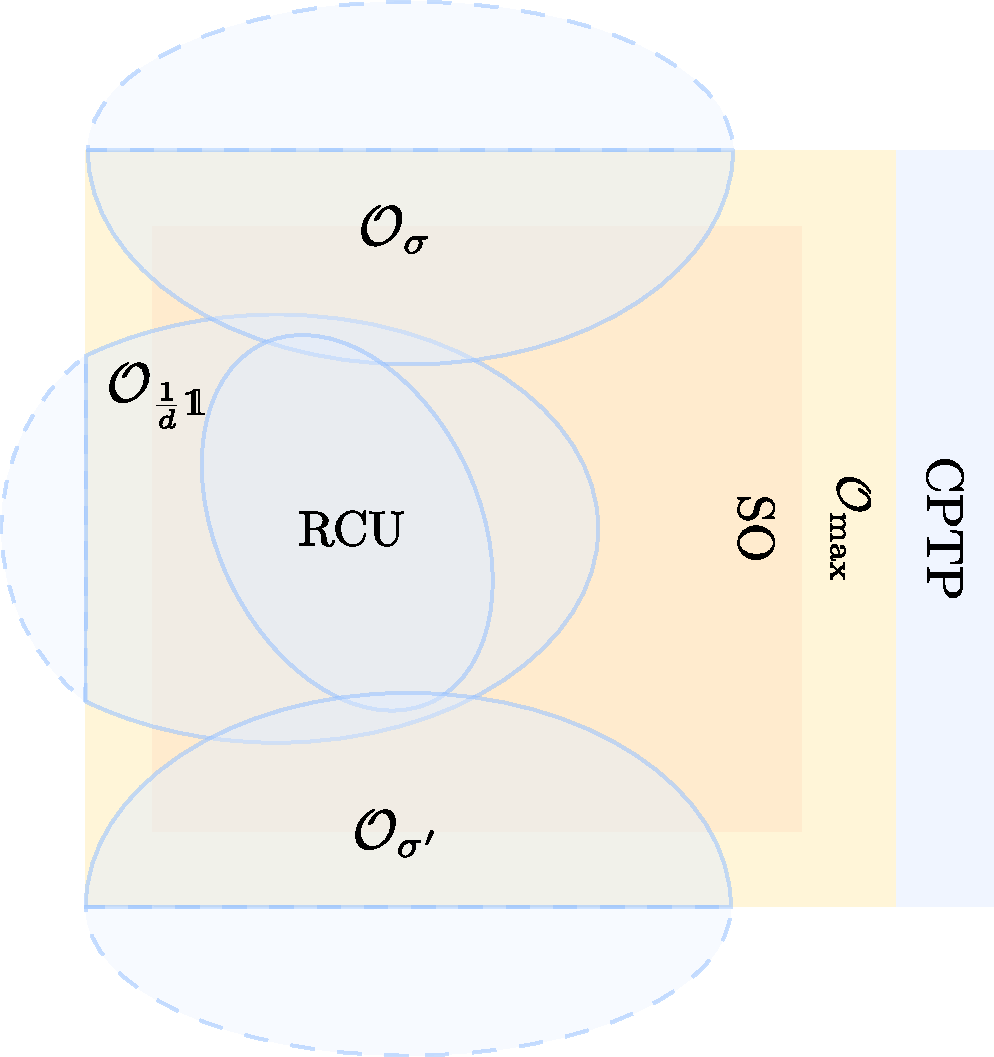
\includegraphics[scale=0.3
        ]{figs/operations.pdf}
    \caption{\textbf{Decomposition of a magic theory $\R$ intro $\sigma$--fragments.} 
	Examples of magic theories ($\so$: Stabilizer operations, $\Omax$: Completely positive-Wigner-preserving operations, $\rcu$: Random Clifford Unitaries -- subclass of $\so$) involve operations denoted by the two yellow regions, with other established magic theories  between them.
    We introduce $\sigma$--fragments $\O_\sigma$ defined for all free states $\sigma$ that cover $\Omax$. 
    Each $\O_\sigma$ is extensible to a set of stochastic maps outside the $\cptp$ operations.
    Within each $\sigma$--fragment $\bmd$--majorisation can be used allowing for tractable approach towards the study of magic state interconversion.
    }
    \label{fig:zoo}
\end{figure}

The zoo of all magic operation classes is summarised in ~\cref{fig:zoo}.
It is clear from the diagram that free operations are in general mapped onto strict subsets of stochastic maps.
This statement, along with more technical properties of the $\sigma$--fragment are discussed in~\cref{app:frag}.
Completely positive-Wigner-preserving operations~\cite{Wang_2019} form the maximal operation class $\Omax$.
This theory of magic is thus covered by $\sigma$--fragments exactly and every other magic theory is contained within this cover.
In particular, the stabiliser operations $\so$ are contained within $\Omax$.

Every  quantum circuit aiming at a given magic state conversion $\rho \longrightarrow \tau$ possesses certain symmetries according to~\cref{thm:frag} that allow us to study the conversion within only certain $\sigma$--fragments that reflect these symmetries.
As a simple example, the dephasing channel
\begin{equation}\label{eq:dephase}
	\Delta(\rho) = \sum_{k \in \mathbb{Z}_d} \ketbra{k}{k}\rho\ketbra{k}{k}
\end{equation}
removes coherent phases in the computational basis and therefore leaves exactly all mixtures of computational basis states invariant.
A noise channel consisting only of such dephasing operations can be fully analysed in the $\sigma$--fragments for the pure computational basis states $\sigma$ as proven in~\cref{app:frag}.

The subdivision of magic theories into $\sigma$--fragments is also powerful because the pre-order $\prec_{\R_\sigma}$ of every $\sigma$--fragment is described by well-behaved majorisation tools, as we establish in the rest of this section.


\subsection{Majorisation}
\label{sec:major}

Majorisation~\cite{cit:marshall} is a collection of powerful tools that has recently found many applications in quantum information theory~\cite{Nielsen_1999, cit:cwiklinski, cit:lostaglio2, cit:gour, cit:gour2, Horodecki_2003, Vallejos_2021}.
It describes the \nick{disorder / non-uniformity} of distributions that undergo stochastic transformations.

To formally state majorisation results, we first denote by $\stoch$ the set of $(d \times d)$ stochastic matrices that preserve the probability vector $\bmd$.
Specifically, for any \emph{$\bmd$--stochastic matrix} $S \in \stoch$, all matrix elements are non-negative, all rows sum to $1$ and $S\bmd = \bmd$.
The set $\stoch$ forms a group under matrix multiplication for any $\bmd$ with positive components.

Majorisation describes quantum thermodynamics exactly in the absence of quantum coherence.
The use of majorisation in this setting provides vital intuition for our purposes.
At any given temperature $\beta^{-1}$, the thermal state $\gamma_\beta$ is thermodynamically the most disordered state. 
Thermal operations are defined as operations that cannot extract energy from the Gibbs state, $\E(\gamma_\beta) = \gamma_\beta$.
Convertibility between states via thermal operations is equivalent to a stochasticity condition on the energy level populations of the states~\cite{cit:lostaglio}.
Informally, there exists a thermal operation $\E$ such that $\tau = \E(\rho)$ if and only if there exists a matrix $S \in \stoch$ such that $\bm{q} = S\bm{p}$, where $\bm{q}, \bm{p}$ and $\bmd$ and the energy level population vectors of $\tau, \rho, \gamma_\beta$ respectively.

Based on this setting, we define $\bmd$--majorisation as follows.
\begin{definition}[\textbf{$\boldsymbol\bmd$--majorisation}]\label{def:dmajor}
    Given $\bmx, \bmy, \bmd \in \reals^d$, such that the components of $\bmd$ are positive, $\bmy$ is said to $\bmd$--majorise $\bmx$, iff there exists a $\bmd$--stochastic matrix $S$ such that $\bmx = S\bmy$.
\end{definition}
We denote this pre-order by $\bmx \prec_{\bmd} \bmy$.
If $\bmd = \frac{1}{d}\bm{1}$, the $d$--dimensional uniform distribution, then $\stoch$ is the set of doubly stochastic matrices and we retrieve the familiar notion of majorisation from entanglement theory~\cite{Nielsen_1999}.

The pre-order imposed by $\bmd$--majorisation admits a numerically efficient reformulation in terms of Lorenz curves.
Let the vector $\bmu^\downarrow$ denote the vector $\bmu \in \reals^d$ with its components arranged in non-increasing order.
\begin{definition}[\textbf{Lorenz curve}]\label{def:lc}
    Let $\bmw, \bmd \in \reals^d$, where the components of $\bmd$ are positive with $D = \sum_{i=1}^d d_i$ and denote by $\widetilde{\bmw} \coloneqq (w_1/d_1, \dots, w_d/\nick{d_d})^T$ the rescaled vector $\bmw$ by $\bmd$.
    
    Finally, denote by $\pi: \mathbb{Z}_d \mapsto \mathbb{Z}_d$ the permutation that sorts $\widetilde{\bmw}$, $(\widetilde{\bmw}^\downarrow)_i = w_{\pi(i)}$ for all $i=1,\dots,d$.
    
    Consider the piecewise linear curve obtained by joining the points $\{(0,0)\} \cup \{ (x_k, \lc{\bmw}{\bmd}(k)) \}_{k=1,\dots,d}$, where
    \begin{equation}\label{eq:lorenz}
        (x_k, \lc{\bmw}{\bmd}(k)) \coloneqq \left( \frac{1}{D}\sum_{i=1}^k d_{\pi(i)}, \sum_{i=1}^k w_{\pi(i)} \right).
    \end{equation}
    We define the set of points on this curve, $\lc{\bmw}{\bmd}(x),\ x \in [0,1]$, as the \emph{Lorenz curve} of vector $\bmw$ with respect to $\bmd$.
\end{definition}
Components $x_k$ are rescaled by $D$ so that comparison of curves with unequal dimensions is possible.
In fact, the Lorenz curves $\lc{\bmw}{\bmd}$ and $\lc{\bmw \otimes \bmd}{\bmd \otimes \bmd}$, where $\otimes$ denotes the Kronecker product, coincide.
Furthermore, a Lorenz curve $\lc{\bmw}{\bmd}(x)$ is always concave in $x$, since it consists of $d$ line segments each with slope $(\widetilde{\bmw}^\downarrow)_i$ for $i=1,\dots,d$ which by definition is a non-increasing sequence.
Finally, the points on the interior of the Lorenz curve that connect line segments of different slopes are in general non-differentiable and we call them\emph{elbows}.

A vector $\bmy$ is said to \emph{$\bmd$--majorise} another vector $\bmx$ if and only if the Lorenz curve $\lc{\bmy}{\bmd}$ lies above Lorenz curve $\lc{\bmx}{\bmd}$, thus reducing $\bmd$--majorisation into a finite set of inequalities.
\begin{theorem}\label{thm:dmajor}
    Let $\bmx, \bmy, \bmd \in \reals^d$, such that the components of $\bmd$ are positive. 
    Then, $\bmx \prec_{\bmd} \bmy$ if and only if $\lc{\bmx}{\bmd}(x) \leq \lc{\bmy}{\bmd}(x)$ for all $x \in [0,1]$ with strict equality at $x=1$.
\end{theorem}
A restatement of the theorem including more equivalent conditions and a proof are provided in~\cref{app:major}.
	


\subsection{Majorisation of quasi-probabilities in $\sigma$--fragments}\label{sec:major_frag}

We can approach any magic theory through a thermodynamic lens, and in doing so we are provided with valuable insights on the structure of the theory. 
Firstly, any free state, for example a stabiliser state, can be viewed as a thermal state $\gamma_\beta$.
Without loss of generality we can always write a quantum state $\sigma$ as a thermal state, $\sigma = \gamma_\beta \coloneqq \frac{1}{\Z_\beta} e^{-\beta H}$ for some $\beta \geq 0$ and Hamiltonian $H$ (either effective or actual)\footnote{Technicalities arise for the case where $\sigma$ is not full rank, but this can be still described via $ \beta \rightarrow 0$ limiting process.}.
We can also view the set of free operations $\O_\sigma$ as a counterpart of thermal operations, in the sense that any operation $\E$ in $\O_\sigma$ preserves state $\sigma$. 

It is then apparent that the pre-order $\prec_{\R_\sigma}$ between the operations in the $\sigma$--fragment follows the rules of $\bmd$--majorisation as outlined in~\cref{sec:major}.
In particular, the pre-order $\prec_{\R_\sigma}$ of the $\sigma$--fragment $\R_\sigma = (\F, \O_\sigma)$ between $d$--dimensional states corresponds to the majorisation pre-order $\prec_{\W{\sigma}}$ between their $d^2$--dimensional Wigner distributions.
For simplicity we shall merge the notation into $\prec_\sigma$, as there is little risk of confusion.

Note that the Wigner components of an $n$--copy state $\rho^{\otimes n}$ can be calculated directly from $\W{\rho}$ by convolution of the distribution with itself,
\begin{equation}
	\W{\rho^{\otimes n}} = \W{\rho}^{\otimes n},
\end{equation}
where $\otimes$ can be interpreted as the usual Kronecker product in the last expression.
We may use the vector notation $\bmw(\rho) = (w(\rho)_i)_{i=1,\dots,d^2}$ for the Wigner distribution, in which case we can express the Kronecker product as
\begin{equation}
	\W{\rho} \otimes \W{\rho} = (w(\rho)_i w(\rho)_j)_{i,j=1,\dots,d^2}.
\end{equation}
The correspondence between the phase space and pure vector representations of the Wigner distribution is discussed more in~\cref{app:cmpairs}.
The vector notation will be useful in the proof of our main result,~\cref{thm:stab_bounds}

Furthermore, we restrict our analysis to $\sigma$--fragments, where $\sigma$ is full-rank.
This is justified as majorisation is continuous between fragments, in the sense that the pre-orders $\prec_\sigma$ and $\prec_{\sigma'}$ are equivalent for states $\sigma$ and $\sigma'$ which are $\epsilon$--close. \nick{CHECK}
Therefore, majorisation analysis is robust under imperfections in the experimental implementation of quantum operations.

In particular, we can always use common noise effects to approximate any $\sigma$--fragment where $\sigma$ is not full-rank by the $\sigma'$--fragment where $\sigma'$ is a noisy approximation of $\sigma$. 
For example, inducing depolarising noise, we can write $\sigma' = (1-\epsilon)\sigma + \epsilon\frac{1}{d}\id$, for some infinitesimal $\epsilon > 0$, so that $\sigma'$ is full-rank and arbitrarily close to $\sigma$.
Important examples of such $\sigma$--fragments include pure stabiliser states which are rank-$1$, e.g. the zero state depicted in~\cref{fig:zero}. 
Operations in such fragments include important stabiliser operations like the replacement channel, $\E(\rho) = \sigma$ for all states $\rho$.

\begin{theorem}\label{thm:sigmamajor}
    Let $\R = (\F, \O)$ be a theory of magic. If $\rho \longrightarrow \tau$  in $\R$ then  $\W{\tau} \prec_\sigma \W{\rho}$ within at least one $\sigma$--fragment.
\end{theorem}
\begin{proof}
Suppose we can convert $\rho$ into $\tau$ in the magic theory. 
Thus there is some $\O_\sigma$ and some $\E \in \O_\sigma$ such that $\E(\rho) = \tau$, and $\E(\sigma)=\sigma$. 
Therefore, the Wigner distribution of this free operation satisfies $\W{\E} \in \stochw$ and $\W{\E}\W{\rho} = \W{\tau}$. 
Since $\sigma$ is full-rank and free, its Wigner distribution is strictly positive in all components, so it directly follows from~\cref{def:dmajor} that $\W{\tau} \prec_{\sigma} \W{\rho}$.
\end{proof}
The converse is in general not true, since stochastic matrices do not necessarily correspond to valid quantum operations.

The result of~\cref{thm:sigmamajor} can be understood as an extension of the idea of a magic monotone, where we replace $\M(\tau) \leq \M(\rho)$ with $\W{\tau} \prec_\sigma \W{\rho}$. 
The physical difference between the two expressions is that the majorisation ordering occurs in a specific $\sigma$--fragment.
Therefore, majorisation constraints can be used to place upper bounds on magic state distillation in a way that allows one to incorporate the physics of the allowed operations -- specifically, it enables us to bound how much magic can be distilled via quantum operations that, for example, preserve the equilibrium state of the system, or via operations that are symmetric about the $Z$-axis of the Bloch sphere.
We discuss distillation upper bounds in detail in~\cref{sec:unital,sec:stab}

This approach can also provide \emph{lower bounds} on distillation, however now more structure about the specific free operations must be included. 
We briefly discuss distillation lower bounds in~\cref{sec:lower_bounds}.

\nick{Mention relative majorisation as a possibility}

\subsection{Lorenz curves of quasi-probabilities in $\sigma$--fragments}
\label{sec:lc}

It is straightforward to construct Lorenz curves for Wigner distributions in any $\sigma$--fragment.
As we have seen in~\cref{thm:sigmamajor}, for any full-rank free state $\sigma$ we have that $\W{\sigma}$ is a strictly positive full-rank probability distribution, and so one can define a corresponding notion of $\bmd$--majorisation on \emph{quasi}--distributions.
We write $\lc{\rho}{\sigma}(x)$ for the Lorenz curve of $\W{\rho}$ with respect to $\W{\sigma}$.
The vector of ratios $\widetilde{\bmw}(\rho|\sigma)$ used to construct the curve is
\begin{equation}
	\widetilde{w}(\rho|\sigma)_i \coloneqq \frac{w(\rho)_i}{w(\sigma)_i},
\end{equation}
and is called the \emph{rescaled} distribution of $\rho$ with respect to $\sigma$.

An example of comparison between different Lorenz curves is provided in~\cref{fig:lctoy}.
The curves in the figure are constructed in the \emph{unital fragment}, i.e. the $\sigma$--fragment defined by the maximally mixed state $\sigma = \frac{1}{d}\id$ whose Wigner distribution is the uniform probability distribution.
\begin{figure}
    \centering
    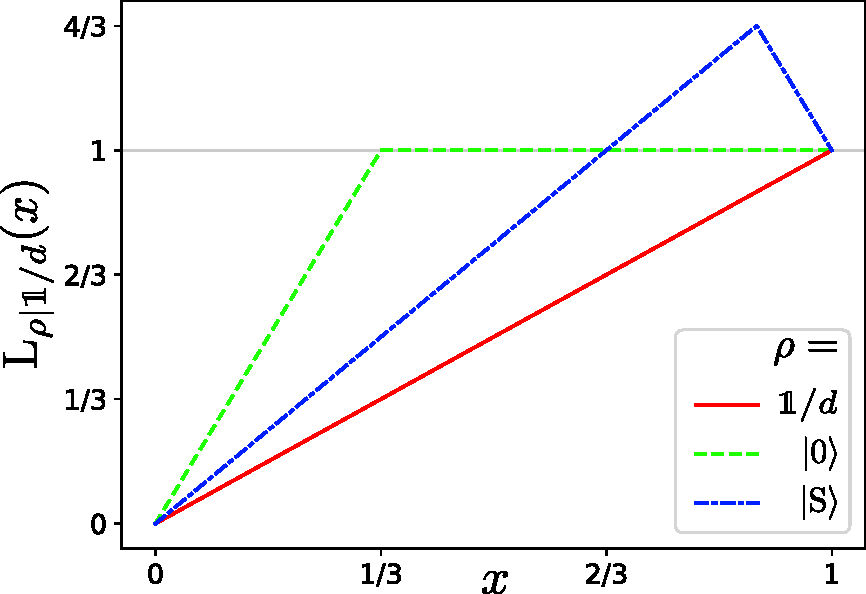
\includegraphics[height=5cm]{figs/lctoy.pdf}
    \caption{\textbf{Quasi-probability Lorenz curve comparison}.
    The Lorenz curves are constructed by the Wigner distributions illustrated in~\cref{fig:wstate_examples} in the unital fragment $\O_{\id/d}$ for $d=3$.
    The maximally mixed state curve is simply the line connecting $(0,0)$ and $(1,1)$.
    There is no operation in $\O_{\id/d}$ that can convert $\ket{\rm{S}}$ to $\ket{0}$, as their Lorenz curves intersect.
    }
    \label{fig:lctoy}
\end{figure}

Normalisation of the Wigner distribution ensures that for all quantum states $\rho$, $\lc{\rho}{\sigma}(x) \geq 0$ and $\lc{\rho}{\sigma}(1) = 1$.
We stress that $0 \leq \lc{\rho}{\sigma}(x) \leq 1$ for all $x \in [0,1]$ if and only if $\rho$ is a positive Wigner state.
As a consequence, checking whether a magic state conversion of the form
\begin{equation}\label{eq:sigma_conv}
	\rho \xrightarrow{\E \in \O_\sigma} \tau
\end{equation} 
is not possible, reduces to the set of constraints
\begin{equation}\label{eq:majbound}
    \lc{\rho}{\sigma}(x) \geq \lc{\tau}{\sigma}(x),\ x\in [0,1],
\end{equation}
due to~\cref{thm:sigmamajor,thm:dmajor}.

We can refine the number of independent constraints stemming from this inequality. 
In fact, there are only as many independent constraints as there are elbows in the Lorenz curve of the target state as shown in~\cref{thm:elbows} in~\cref{app:frag}.
However, in principle any one location $x$ provides a valid constraint leading to some upper distillation bound, while optimising over the location would provide the strictest bound.
In particular, we establish the \emph{first elbow constraint} which we use in~\cref{sec:unital,sec:stab} explicitly.
\begin{lemma}
	Consider a magic state interconversion as in~\cref{eq:sigma_conv}, where we denote by $(x_0, L_0)$ and $(x'_0, L'_0)$ the first elbow coordinates of the initial and target states respectively.
	If $x_0 < x'_0$, then it holds that
\begin{equation}\label{eq:first_elb_bound1}
	\frac{L_0}{x_0} \geq \frac{L_0'}{x_0'}.
\end{equation}
\end{lemma}
\begin{proof}
	Consider the Lorenz curve constraint at $x = x_0$,
\begin{equation}
	\lc{\rho}{\sigma}(x_0) \geq \lc{\tau}{\sigma}(x_0).
\end{equation}
Since $x_0 < x'_0$, we can find the target state Lorenz curve coordinate $L'_\star$ at location $x = x_0$ by interpolating between the origin and the target state's first elbow, 
\begin{equation}
	L'_\star = \frac{x_0}{x'_0}L'_0.
\end{equation}
We need $L_0 \geq L_\star'$ and rearranging we get~\cref{eq:first_elb_bound1}.
\end{proof}

We can now turn the attention from the first elbow to the peak of the Lorenz curve to associate it directly with the magic monotone of mana, and equivalently the sum-negativity of a quantum state. 
This holds independently of the particular $\sigma$--fragment one works in and as a result it becomes apparent that mana provides a weaker condition than majorisation for all magic state interconversions.

We first show that the Lorenz curve maximum of state $\rho$ is independent of the $\sigma$--fragment and directly related to its sum-negativity.
\begin{lemma}\label{lem:lcmax}
	Given a quantum state $\rho$, the maximum of its Lorenz curve $\lc{\rho}{\sigma}$ is independent of the $\sigma$--fragment and is equal to $1+\sn{\rho}$.
\end{lemma}
\begin{proof}
	We may use the vector notation of the Wigner distributions $\bmw(\rho)$ and $\bmw(\sigma)$.
	We choose the component indexing so that the rescaled distribution 
	\begin{equation}
		\widetilde{\bm{w}}(\rho|\sigma) \coloneqq \left(\frac{w(\rho)_1}{w(\sigma)_1}, \dots, \frac{w(\rho)_{d^2}}{w(\sigma)_{d^2}} \right)^T,
	\end{equation}
	is sorted, $\widetilde{\bm{w}} = \widetilde{\bm{w}}^\downarrow$.
	Note that all components of $\bmw(\sigma)$ are positive, so $\widetilde{w}_i \geq 0$ if and only if $w(\rho)_i \geq 0$ for any $i=1,\dots,d^2$.
	
	Let $i_\star$ be the index of the smallest non-negative component of $\widetilde{\bm{w}}^\downarrow$.
	Then, $w(\rho)_i < 0$ if and only if $i > i_\star$, so the maximum of Lorenz curve $\lc{\rho}{\sigma}(x)$ takes the value 
	\begin{equation}
		\lc{\rho}{\sigma}(x_{i_\star}) = \sum_{i=1}^{i_\star} w(\rho)_i,
	\end{equation}
	and is achieved at
	\begin{equation}\label{eq:maxloc}
		x_{i_\star} \coloneqq \sum_{i=1}^{i_\star} w(\sigma)_i.
	\end{equation}

	The location of the maximum ($x=x_{i_\star}$) varies from fragment to fragment, but its value is independent of $\sigma$,
	\begin{equation}
		\lc{\rho}{\sigma}(x_{i_\star})
		= \sum\limits_{\bmx: \W[\bmx]{\rho} \geq 0} \W[\bmx]{\rho}
		= 1 + \sn{\rho}.
	\end{equation}
	
\end{proof}

We can therefore view mana as just one feature of the Lorenz curve, namely its maximum value. 
Conversely, it is now clear that the maximum of the Lorenz curve acts as a valid magic monotone.
\begin{theorem}\label{thm:bounds}
    Given a magic state conversion $\rho \longrightarrow \tau$, the majorisation condition is stronger than the mana condition in every $\sigma$--fragment.
\end{theorem}
\begin{proof}
    The maximum of the Lorenz curve of a state $\rho$ is independent of the $\sigma$--fragment due to~\cref{lem:lcmax}, and can be expressed as an increasing function of mana,
    \begin{equation}
        \max_{x\in[0,1]}{\lc{\rho}{\sigma}(x)} = 1 + \sn{\rho} = \frac{1}{2} \left( 1 + e^\mana{\rho} \right).
    \end{equation}
    Therefore, the majorisation bound
    \begin{equation}
    	\lc{\rho}{\sigma}(x) \geq \lc{\tau}{\sigma}(x),\ x\in[0,1]
    \end{equation}
    implies the order $\max_{x\in[0,1]}{\lc{\rho}{\sigma}(x)} \geq \max_{x\in[0,1]}{\lc{\tau}{\sigma}(x)}$, hence the mana condition $\mana{\rho} \geq \mana{\tau}$.
\end{proof}

The area $\A_\sigma(\rho)$ between the curve $L_{\rho|\sigma}$ and the line $y=1$ is also a resource monotone in the $\sigma$--fragment. 
This is clear because for any state conversion like~\cref{eq:sigma_conv}, the Lorenz curve $L_{\tau|\sigma}$ is lower than $L_{\rho|\sigma}$, hence $\A_\sigma(\E(\rho)) \leq \A_\sigma(\rho)$.
It cannot be directly expressed in terms of mana, as it depends on positive Wigner components as well.

In~\cref{sec:unital,sec:stab}, we study majorisation constraints on magic distillation arising in different fragments. 
For this reason, we define the $n$--copy, $\epsilon$--noisy Strange state,
\begin{equation}\label{eq:noisysn}
    \rho_{\rm{S}}(\epsilon)^{\otimes n} \coloneqq \left[ (1 - \epsilon) \ket{\rm{S}}\bra{\rm{S}} + \epsilon \frac{1}{3}\id \right]^{\otimes n},
\end{equation}
in $\O_\sigma$, where the pure magic state $\ket{\rm{S}}$ is induced with depolarising noise. 
Its Wigner distribution is visualised in~\cref{fig:strange}.

We refer to parameter $\epsilon$ as \emph{noise level} to avoid confusion with the error rate $\delta$, a term commonly used in the literature to denote that the distilled state has a marginal overlap of at least $1-\delta$ with the desired magic state.
In our case the error rate of the state in~\cref{eq:noisysn} would be $\delta = \frac{2}{3}\epsilon$.

At $\epsilon=0$, the Strange state is a qutrit magic state of maximal sum-negativity / mana~\cite{cit:veitch2} and therefore acts as an ideal distillation target, analogous to a Bell state in bipartite entanglement theory.
The Strange state is exceptionally symmetric under Clifford transformations and as a result there exists a \emph{twirling} protocol, discussed in detail in~\cite{cit:prakash,cit:prakash2}, allowing for the conversion of any noisy magic state to the form of~\cref{eq:noisysn} via Cliffords.

In~\cref{fig:lcs}, we illustrate the Lorenz curve $\lc{\rho_{\rm{S}}}{\sigma}$\footnote{Hereinafter, we may omit obvious variable dependencies like $\epsilon$ and $n$ for clarity} of pure and noisy $n$--copy Strange states in some thermal $\sigma$--fragment.
Due to~\cref{lem:lcmax}, it is clear that the curves peak at $1 + \sn{\rho_{\rm{S}}(\epsilon)^{\otimes n}}$.
\begin{figure}
    \centering
    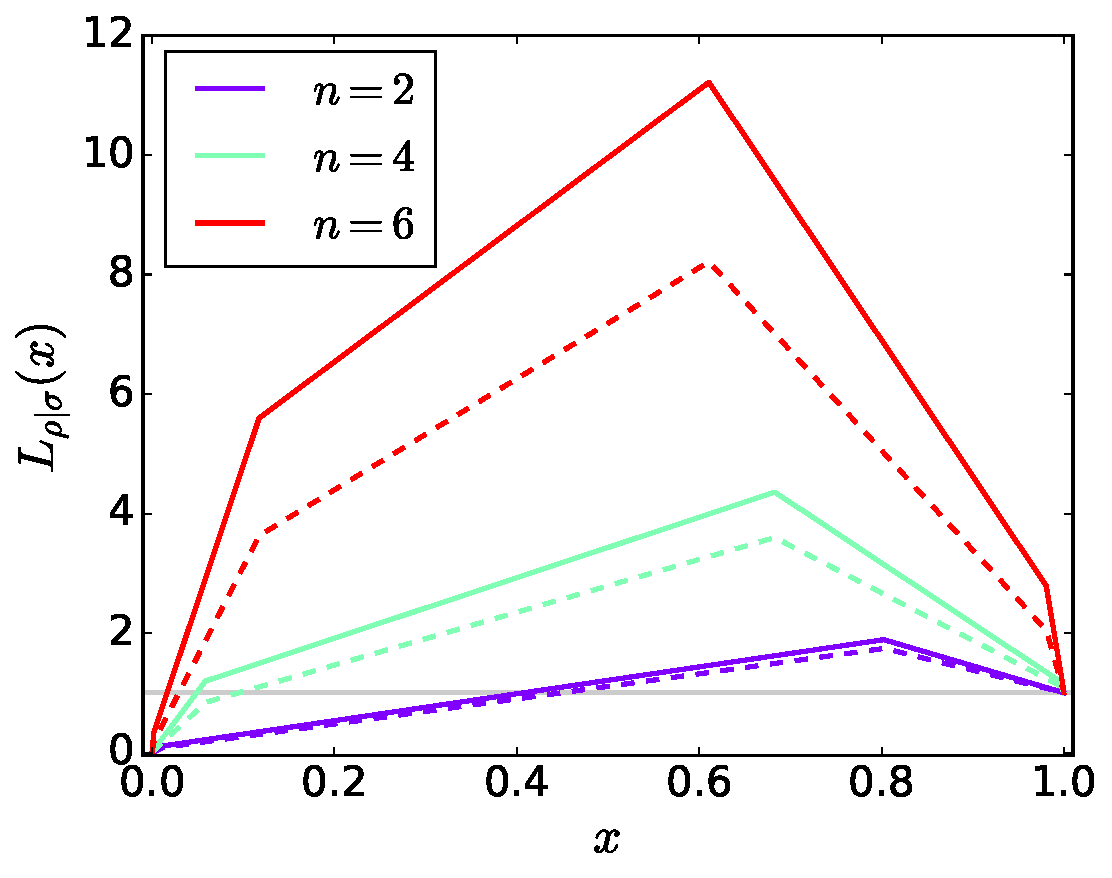
\includegraphics[height=5cm]{figs/lc_strange.pdf}
    \caption{\textbf{A `heretical' family of Lorenz curves.} Traditionally, Lorenz curves are monotone increasing cumulant functions that reach a maximum value of $1$. In contrast, Lorenz curves for magic states break through the value of $L(x)=1$ due to the presence of negativity in the associated quasi-probability distribution. The above family of curves correspond to multiple copies of noisy Strange states $\rho_{\rm{S}}(\epsilon)^{\otimes n}$ for $n=1,2,3,4$ within a particular stabilizer fragment. Solid lines represent pure Strange states, while dashed lines represent noisy Strange states with depolarising noise $\epsilon = 0.1$.
    }
    \label{fig:lcs}
\end{figure}

\section{Magic in the unital fragment}
\label{sec:unital}

The unital fragment encompasses the circuits which preserve the maximally mixed state ($\id/d$) and so it includes many important families of circuits.

MSD circuits in principle consist of bulk sequences of random Clifford unitaries ($\rcu$)~\cite{cit:bravyi}, depicted in~\cref{fig:zoo}.
Operations in $\rcu$ can be expressed as
\begin{equation}
    \E(\rho) = \sum_i p_i U_i \rho U_i^\dagger,\ U_i \in \cal{C}_d.
\end{equation}
Depending on the symmetries of such operations, a Clifford sequence may belong in other $\sigma$--fragments as well.
In such a case, the majorisation condition~(\ref{eq:majbound}) needs to be checked in the $\sigma$--fragments that reflect all symmetries of the operation sequence.

In general, noisy circuits are well-described by the unital fragment.
To see this, consider incorporating noisy channels in the circuit, for example dephasing channels as in~\cref{eq:dephase} defined in different bases.
This process destroys the circuit symmetries, except for the invariance of the maximally mixed state.
Dephasing and bit-flip error channels are examples of the many error-inducing channels that respect the unital symmetry. \nick{Expand on significance of unital fragment}
\null\\

We consider the task of purifying $n$ copies of a noisy Strange state $\rho_{\rm{S}}(\epsilon)^{\otimes n}$ as given in~\cref{eq:noisysn} into a smaller number of copies $n'$ of a less noisy strange state $\rho_{\rm{S}}(\epsilon')^{\otimes n'}$, with $\epsilon' < \epsilon$ and $n' \leq n$,
\begin{equation}\label{eq:sudist}
	\rho_{\rm{S}}(\epsilon)^{\otimes n} \longrightarrow \rho_{\rm{S}}(\epsilon')^{\otimes n'} \otimes \left( \frac{1}{3}\id \right)^{\otimes (n-n')},
\end{equation}
where all copies $n, n', n - n'$ are even.
Since the state $\id / 3$ is free, tensoring in copies of it does not affect the distillation process.
The distillation rate $R \coloneqq n'/n$ for this process will in general depend on the noise levels, $R = R(\epsilon, \epsilon')$ and our task is to provide it with an upper bound.

The Lorenz curve $\lc{\rho_{\rm{S}}}{\id/3}$, for some general noise parameter $\epsilon$ and number of copies $n$, is defined at $9^n$ points between $0$ and $1$.
The exact expressions for the coordinates of these points can take $8$ different forms, depending on whether the noise level $\epsilon$ is greater or less than $\frac{3}{7}$, the parity of the number of copies $n$ is even or odd and the location relative to the curve peak is on the left hand side (LHS -- including the curve peak) or right hand side (RHS) of the curve peak.
The full details for the construction of all Lorenz curve forms are provided in~\cref{app:lcsu_technical}.

Here we focus on the comparison of the first elbow (which lies in the LHS part) of Lorenz curves with even copies $n, n'$ and low noise levels ($\epsilon' < \epsilon \leq 3/7$).

The Wigner distribution of the 1-copy, $\epsilon$--noisy Strange state can be written as 
\begin{equation}
	\W[\bmx]{\rho_{\rm{S}}(\epsilon)} = (1-\epsilon)\W[\bmx]{\ketbra{\rm{S}}} + \epsilon\W[\bmx]{\frac{1}{3}\id},
\end{equation}
so we get positive components
\begin{equation}
	u(\epsilon) \coloneqq \frac{1}{6} -\frac{1}{18}\epsilon
\end{equation}
at the 8 phase space points $\bmx \in \cal{P}_3 \setminus \{\bmo\}$ and a negative component
\begin{equation}
	- v(\epsilon) \coloneqq - \left( \frac{1}{3} -\frac{4}{9}\epsilon \right)
\end{equation}
at the origin $\bmx = \bmo$.

The rescaled distribution in the unital fragment simply is 
\begin{equation}
	\widetilde{\rm{W}}_{\rho_{\rm{S}}|\frac{1}{3}\id}(\bmx) = \frac{\W[\bmx]{\rho_{\rm{S}}}}{\W[\bmx]{\frac{1}{3}\id}} = d\W[\bmx]{\rho_{\rm{S}}},
\end{equation}
so ordering the rescaled distribution is equivalent to ordering $\W{\rho_{\rm{S}}}$.

The component values and multiplicities ($m_i$) in the $n$--copy case are 
\begin{align}
	m_i &= 8^{2i}\binom{n}{2i}, \\
	w(\rho_{\rm{S}})_i &= u^{2i}(-v)^{n-2i}, \\
	w(\id/3)_i &=  \frac{1}{9^n},
\end{align}
where index $i$ runs through $0,\dots,\frac{n}{2}$.
This is derived in~\cref{app:lcsu_coord_elb}.

It is readily seen that the maximum Wigner component is achieved when $i=0$, so the corresponding multiplicity and Wigner component are $m_0 = 1$, $w(\rho_{\rm{S}})_0 = v^n$.
The first elbow coordinates therefore can be expressed as
\begin{equation}\label{eq:first_elb_coords}
	(x_0, L_0) = (m_0\hspace{2pt} w(\id/3)_0,\ m_0\hspace{2pt} w(\rho_{\rm{S}})_0) = \left(\frac{1}{9^n}, v^n \right)
\end{equation}

The first elbow of the target state is located at $x'_0 = \frac{1}{9^{n'}} > x_0$, so we can use the first elbow condition,
\begin{equation}\label{eq:first_elb_bound2}
	\frac{L_0}{x_0} \geq \frac{L_0'}{x_0'},
\end{equation}
to compute analytical distillation bounds for distillation rate $R = R(\epsilon, \epsilon') \coloneqq n'/n$ in the unital fragment.
We substitute coordinates from~\cref{eq:first_elb_coords} appropriately in~\cref{eq:first_elb_bound2} to get
\begin{equation}
	R \leq \frac{\ln{(3-4\epsilon)}}{\ln{(3-4\epsilon')}}.
\end{equation}

Specifically for the problem of distilling pure magic states ($\epsilon'=0$), we obtain an upper bound in the unital fragment given by
\begin{equation}
	R \leq 1 + \frac{\ln (1 - \frac{4}{3} \epsilon)}{\ln 3}.
\end{equation}

Similar upper bounds on distillation rates for qudits of odd prime dimension include the mana bound~\cite{cit:veitch} and the max--thauma bound~\cite{Wang2020} which is defined via a semi-definite program, but possesses properties that allow for an easy comparison with our bound.
The mana bound can be directly calculated as
\begin{equation}
	R \leq \frac{\mana{\rho_{\rm{S}}(\epsilon)}}{\mana{\rho_{\rm{S}}(0)}} = 1 + \frac{\ln \left(1 - \frac{8}{15}\epsilon \right)}{\ln \frac{5}{3}}.
\end{equation}
Using the max--thaum properties of super-additivity and vanishing at free states, we obtain
\begin{align}
	&\theta_{\rm{max}}(\rho_{\rm{S}}(\epsilon)) \geq (1-\epsilon) \theta_{\rm{max}}(\ketbra{\rm{S}}) + \epsilon \theta_{\rm{max}}\left(\frac{1}{3}\id \right) = \nonumber\\
	&(1-\epsilon) \theta_{\rm{max}}(\rho_{\rm{S}}(0)),
\end{align}
so that for a deterministic single-copy distillation process, an initial number of copies $n \geq \theta_{\rm{max}}(\tau) / \theta_{\rm{max}}(\rho) \geq 1-\epsilon$ is required.
Therefore, the max--thauma bound for the pure Strange state distillation process can get as tight as
\begin{equation}
	R = \frac{1}{n} = \frac{\theta_{\rm{max}}(\rho_{\rm{S}}(\epsilon))}{\theta_{\rm{max}}(\rho_{\rm{S}}(0))} \leq 1-\epsilon.
\end{equation}

Both the mana and the max--thauma bounds are looser than the majorization bound we derived via the first elbow constraint as illustrated in~\cref{fig:distill_bounds}.
\begin{figure}[t]
    \centering
    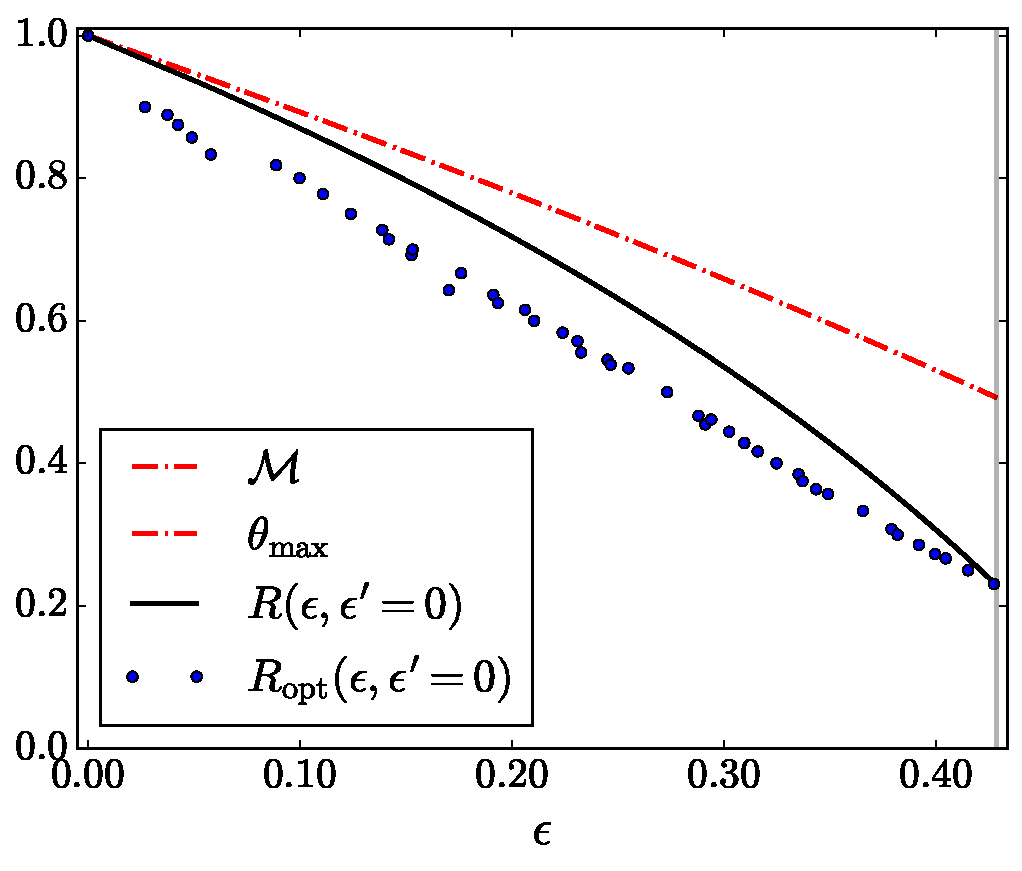
\includegraphics[scale=0.5]{figs/distill_bounds.pdf}
    \caption{\textbf{Distillation bounds in the unital fragment.} Distillation bounds obtained by majorisation, mana and the line $1-\epsilon$ (tightest bound of max--thauma) are plotted for $\epsilon' = 0$, up to noise level $\epsilon = 3/7$.
    Majorisation consistently provides stricter rates than mana and max--thauma.
    }
    \label{fig:distill_bounds}
\end{figure}

\section{Magic bounds in arbitrary stabiliser fragments}
\label{sec:stab}

We now generalise the approach taken in the previous section and consider bounds on magic distillation for an arbitrary stabiliser fragment, $\R_\sigma$ where $\sigma$ is any quantum state $\sigma \in \stab$.
In other words, we consider those bounds on distillation that apply when the free operations have $\sigma$ as a fixed point.

These bounds can be interpreted in two different ways: on one hand they can be viewed as a family of upper bounds parameterized by a stabiliser state $\sigma$, on the other we can associate $\sigma$ to actual hardware limitations or to biased noise models in which it is an equilibrium state of some kind. 
Without loss of generality, we can always write a stabiliser state $\sigma$ as a Gibbs state $\sigma = \gamma_\beta \coloneqq \frac{1}{\Z_\beta} e^{-\beta H}$ for some $\beta \geq 0$ and Hamiltonian $H$ as discussed in~\cref{sec:major_frag}.

We focus on the distillation process
\begin{equation}\label{eq:stdist}
	\rho_{\rm{S}}(\epsilon)^{\otimes n} \longrightarrow \rho_{\rm{S}}(\epsilon')^{\otimes n'} \otimes \sigma^{\otimes (n-n')},
\end{equation}
where the noisy Strange state is given in~\cref{eq:noisysn} and we highlight again that any magic state can be transformed to this form via Clifford operations.
Notice that tensoring in copies of $\gamma_\beta$ does not affect the process, since the state is free.
In the following result, all copies $n, n', n - n'$ are even with $n > n'$, and $\epsilon'=0$, but the bounds are easily generalised to odd numbers of copies and $\epsilon'$ such that $0 < \epsilon' < \epsilon$. 
Finally, we assume a range of initial noise levels, $\epsilon \leq 3/7$, so that the largest Wigner component of the 1-copy noisy magic state is negative.
The numerical value of $3/7$ is higher than corresponding values of relevant existing distillation protocol error thresholds~\cite{cit:bravyi,cit:prakash}.

Given this context, we now provide the following result on bounding the distillation rate $R = R(\epsilon, \epsilon', \beta) \coloneqq \frac{n'}{n}$ of the process in~\cref{eq:stdist}.
We also write $R(\epsilon, \beta) = R(\epsilon, \epsilon'=0, \beta)$.
The bounds depend on the free energy $F_\beta$ of state $\sigma$,
\begin{equation}
	F_\beta \coloneqq \tr[H \sigma] - \beta^{-1}S(\sigma) = -\beta^{-1}\log{\Z_\beta},
\end{equation}
where the von Neumann entropy is $S(\sigma) \coloneqq -\tr[\sigma\log{\sigma}]$.

\begin{figure}[t!]
    \centering
    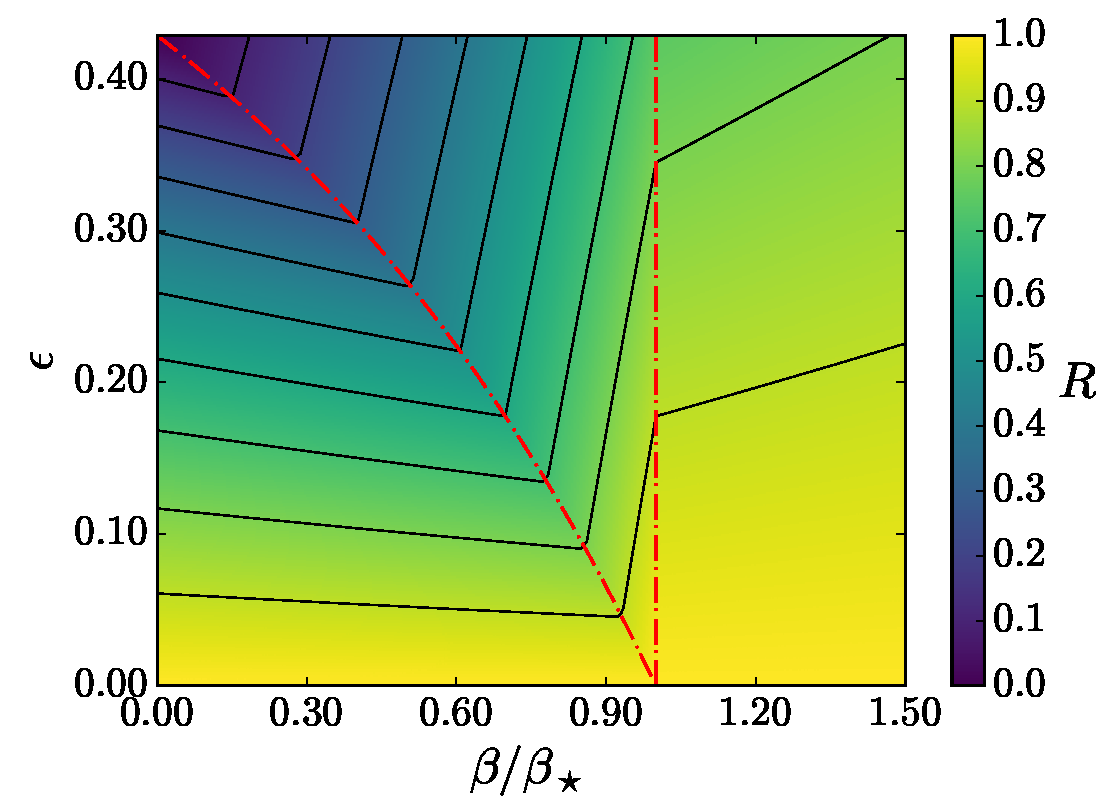
\includegraphics[scale=0.55]{figs/rate_scatter.pdf}
    \caption{\textbf{Bounds on magic distillation rates $R(\epsilon, \beta)$ within stabiliser fragments.}
    The vertical dashed line is the `Landauer-like' temperature threshold $\beta_\star$ and the diagonal dashed curve corresponds to the noise threshold $\epsilon_\star (\beta)$ at every $\beta \leq \beta_\star$. The unital fragment corresponds to the $\beta =0 $ line.
    }
    \label{fig:rate_contour}
\end{figure}

\begin{theorem}\label{thm:stab_bounds}
	Let $\sigma$ be a qutrit stabiliser state, given by $\sigma = \frac{1}{\Z} e^{-\beta H}$ with $H$ having eigenvalues $E_0 \le E_1 \le E_2$, and where $\beta$ is an (effective) inverse temperature for the state. 
We define
\begin{equation}
	\beta_\star \coloneqq \frac{1}{E_2 - E_0} \ln{2}
\end{equation}
and for $\beta \leq \beta_\star$, we define a threshold noise level
\begin{equation}
	\epsilon_{\star}(\beta) \coloneqq 3 - \dfrac{18}{8-e^{(E_2 - E_0)\beta}}.
\end{equation}
Then any distillation rate $R(\epsilon, \beta)$ in the $\sigma$--fragment of a magic theory is bounded as follows:\\
If $\beta \leq \beta_{\star}$ and $\epsilon  \leq \epsilon_{\star}$,
\begin{equation}
	R(\epsilon,\beta) \leq 1 + \frac{\ln{\left( 1 - \frac{4}{3}\epsilon \right)}}{\beta (E_0 - F_\beta)}.
\end{equation}
If $\beta \leq \beta_{\star}$ and $\epsilon_{\star} < \epsilon$, then
\begin{equation}
	R(\epsilon, \beta) \le 1 + \frac{\ln{\left(1-\frac{1}{3}\epsilon \right)} - (E_2 - E_0)(\beta_{\star} - \beta)}{\beta (E_0 - F_\beta)}.
\end{equation}
Otherwise if $\beta > \beta_{\star}$,
\begin{equation}
	R(\epsilon, \beta) \leq  1+ \frac{\ln{\left(1-\frac{1}{3}\epsilon \right)}}{-\ln{2} + \beta (E_2 - F_\beta)}.
\end{equation}
\end{theorem}
A few comments can be given on this result. 
Firstly, the specific numerical factors in $\epsilon_\star$ are a result of our choice of magic state. 
Secondly, these bounds are derived based on analysis of only a part of the Lorenz curves and can be improved via a finer analysis. 
This is apparent by simple numerical calculations on the entirety of the curves.
Specifically, the existing bounds follow by considering the dominant terms in the rescaled Wigner distribution and do not, for example, take into account the Lorenz curve's peak structure. 
Finally, it is striking that we obtain a Landauer-like condition with a characteristic temperature $kT_\star \ln 2 = E_2 - E_0$, where $kT_\star = \beta_\star^{-1}$. 
It is unclear whether this points to a generic feature that can be directly related to fundamental thermodynamic relations, such as the erasure cost of a single bit being $kT \ln 2$. 
Given that we work with qutrits this seems surprising, but does deserve further study.

\begin{proof}
	We provide the full proof here, with some technical details pushed to~\cref{app:lcst_technical}.\\

Let $\displaystyle \sigma = e^{-\beta H} / \Z_\beta$ be a stabiliser state, where $\beta \geq 0$ and $H = E_0 \ketbra{0} + E_1 \ketbra{1} + E_2 \ketbra{2}$, with $E_k \geq 0$.
Its eigen-decomposition can be written as 
\begin{equation}
	\sigma = \frac{e^{-\beta E_0}}{\Z_\beta} \ketbra{\varphi_0} + \frac{e^{-\beta E_1}}{\Z_\beta} \ketbra{\varphi_1} + \frac{e^{-\beta E_2}}{\Z_\beta} \ketbra{\varphi_2},
\end{equation}
where $\{\ket{\varphi_k}\}$ are pure, orthonormal stabiliser states. 
Therefore, there exists a Clifford operation that maps $\sigma$ to $\gamma_\beta$, where 
\begin{equation}
\gamma_\beta = \frac{e^{-\beta E_0}}{\Z_\beta} \ketbra{0} + \frac{e^{-\beta E_1}}{\Z_\beta} \ketbra{1} + \frac{e^{-\beta E_2}}{\Z_\beta} \ketbra{2}.
\end{equation}
\nick{Prove this carefully}

This Clifford operation permutes the Hamiltonian eigenvalues on the phase space, so that the negative component $-v$ of $\rho_S(\epsilon)$ can lie on the same point on the phase space as any of the eigenvalues.
For this reason, we impose no order between the eigenvalues, but simply choose $E_0$ as the eigenvalue that is associated with the state negativity and denote the highest energy by $E_{\rm{max}} \coloneqq \max{\{E_0, E_1, E_2\}}$.

The Wigner distribution of state $\gamma_\beta$ can be seen as the ensemble average of the distributions of the computational basis states,
\begin{align}
	\W[\bmx]{\gamma_\beta} &= \sum\limits_{k=0}^2 \frac{e^{-\beta E_k}}{\Z_\beta}\W[\bmx]{\ketbra{k}} \\
	&= \sum\limits_{k=0}^2 \frac{e^{-\beta E_k}}{\Z_\beta} \delta_{x_0, k} = \frac{e^{-\beta E_{x_0}}}{3\Z_\beta},
\end{align}
for all $\bmx \in \cal{P}_3$. 
All Wigner components are strictly positive, therefore the pre-order $\prec_{\gamma_\beta}$ is always well-defined.

Our aim is to obtain a distillation bound for~\cref{eq:stdist} which depends on variables $n, n', \epsilon, \epsilon'$ as well as $\beta$.
In the analysis that follows, we again drop obvious variable dependencies for clarity.

We construct the Strange state rescaled distribution 
\begin{equation}
	\widetilde{\rm{W}}_{\rho_{\rm{S}}|\gamma}(\bmx) = \frac{\W[\bmx]{\rho_{\rm{S}}}}{\W[\bmx]{\gamma}},
\end{equation}
which attains four distinct values on the phase space, naturally splitting it into four regions as illustrated in the~\cref{fig:pd_split_thermal}.
\begin{figure}[h]
    \centering
    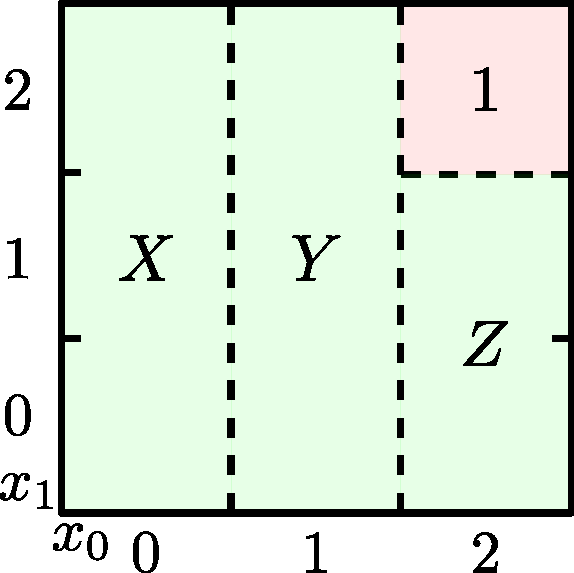
\includegraphics[scale=0.5]{figs/pd_split_thermal.pdf}
    \caption{\textbf{Qutrit phase space regions with different rescaled values.}
    The rescaled distribution attains a unique value in each of the four regions, given by $3\Z \times$ the value depicted in the region, according to~\cref{eq:bmw_rescaled}.
    }
    \label{fig:pd_split_thermal}
\end{figure}

The component values and multiplicities of the relevant distributions in the four distinct regions are summarised by the following component and multiplicity vectors,
\begin{align}
	\bmm &\coloneqq (1,2,3,3), \\
	\bmw(\rho_{\rm{S}}) &\coloneqq (-v, u, u, u), \\
	\bmw(\gamma) &\coloneqq \frac{1}{3\Z} \left( e^{-\beta E_0}, e^{-\beta E_0}, e^{-\beta E_1}, e^{-\beta E_2} \right), \\
	\bmw(\rho_{\rm{S}} | \gamma) &\coloneqq 3\Z \left( -v e^{\beta E_0}, u e^{\beta E_0}, u e^{\beta E_1}, u e^{\beta E_2} \right). \label{eq:bmw_rescaled}
\end{align}

Using this notation, the component values and multiplicities of the $n$--copy distributions can be readily provided by~\cref{lem:ncopycomponents} in~\cref{app:cmpairs}.
They are parametrised by three independent components $i,j,k$, with sum $\alpha \coloneqq i+j+k \leq n$.
The $n$--copy multiplicity is given by
\begin{equation}
	m_{ijk} = \frac{n!}{i!j!k!(n-\alpha)!} 2^i 3^j 3^k,
\end{equation}
while the distribution values that correspond to the same index triplet $(i,j,k)$ are given by
\begin{align}
	w(\rho_{\rm{S}})_{ijk} &= (-v)^{n-\alpha} u^{\alpha}, \\
	w(\gamma)_{ijk} &= (3\Z)^{-n} e^{-\beta (n-\alpha)E_0} e^{-\beta ( i E_0 + j E_1 + k E_2 )}, \\
	w(\rho_{\rm{S}} | \gamma)_{ijk} &= (3\Z)^{n} (-v)^{n-\alpha} u^{\alpha} e^{\beta (n-\alpha)E_0} e^{\beta ( i E_0 + j E_1 + k E_2 )}.
\end{align}

In order to construct the $n$--copy Lorenz curve $\lc{\rho_{\rm{S}}^{\otimes n}}{\gamma}$ we need to sort the components of the $n$--copy rescaled distribution, $w(\rho_{\rm{S}} | \gamma)_{ijk}$ in decreasing order.
In particular, to find the coordinates of the first elbow $(x_0, L_0)$, we need to evaluate the maximum rescaled component,
\begin{align}
	&\bmw(\rho_{\rm{S}} | \gamma)_{\rm{max}} \coloneqq \label{eq:max_slope}\\
	&(3\Z)^{n} \max\limits_{i,j,k}\Big\{ (-v)^{n-\alpha} u^{\alpha} e^{\beta (n-\alpha)E_0} e^{\beta ( i E_0 + j E_1 + k E_2 )} \Big\}, \nonumber
\end{align}
where $0 \leq i,j,k \leq n$ and $\alpha \coloneqq i+j+k \leq n$.
Notice that for $0 \leq \epsilon \leq 3/7$, we have $v \geq u$. 
We assume that $n$ is even, so that we need the sum $\alpha = i+j+k$ to be even for the expression to be positive. 
The following analysis is similar if $n$ is chosen to be odd.

Given an even value for the sum $\alpha$, the term $v^{n-\alpha} u^{\alpha} e^{-\beta (n-\alpha)E_0}$ is fixed, so the expression is maximised by setting the coefficient of the highest energy $E_{\rm{max}}$ equal to $\alpha$.
Hence, we have
\begin{align}
	&\bmw(\rho_{\rm{S}} | \gamma)_{\rm{max}} = \nonumber\\
	&(3\Z)^{n} v^n e^{n\beta E_0}\max\limits_{\substack{\alpha = 0,2, \\ \dots,n-2,n}}{\Big\{ \left( \frac{u}{v} e^{\beta (E_{\rm{max}} - E_0)} \right)^{\alpha} \Big\}}.
\end{align}
If the expression $\frac{u}{v} e^{\beta (E_{\rm{max}} - E_0)}$ is less than $1$ then the maximum occurs at $\alpha=0$, otherwise the maximum occurs at $\alpha = n$. To determine this transition we set
\begin{equation}\label{eq:noise_transition}
	\frac{u(\epsilon)}{v(\epsilon)} e^{\beta (E_{\rm{max}} - E_0)} \coloneqq \frac{3-\epsilon}{6-8\epsilon} e^{\beta (E_{\rm{max}} - E_0)} = 1.
\end{equation}
We want to find in which cases there exists a threshold noise level $\epsilon_\star$ at which the transition in~\cref{eq:noise_transition} occurs.
If $E_{\rm{max}} = E_0$, namely if the state negativity lies in the same phase space region as the highest energy, this threshold is constant in temperature and given by $\epsilon_{\star} = 3/7$. 
Otherwise, there is a threshold temperature value $\beta_\star$ given by
\begin{equation}
	\beta_{\star} \coloneqq \frac{1}{E_{\rm{max}} - E_0} \ln2.
\end{equation}
Below the threshold, $0 \leq \beta \leq \beta_\star$, the transition is well defined and the threshold noise level at which it occurs is given by
\begin{equation}
	\epsilon_{\star}(\beta) := 3 - \dfrac{18}{8-e^{(E_{\rm{max}} - E_0)\beta}}.
\end{equation}
This encompasses the case $E_{\rm{max}} = E_0$.
For $\beta > \beta_\star$, we have
\begin{equation*}
	\frac{3-\epsilon}{6-8\epsilon} e^{\beta (E_{\rm{max}} - E_0)} > \frac{3-\epsilon}{6-8\epsilon} 2 \geq \frac{1}{2}2 = 1,
\end{equation*}
so there is no transition and we set $\epsilon_\star = 0$.

The maximum rescaled component can then be expressed as
\begin{equation*}
\bmw(\rho_{\rm{S}} | \gamma)_{\rm{max}} =
	\begin{cases}
		(3\Z)^{n} v^n e^{n\beta E_0}, &\epsilon \leq \epsilon_{\star},\ \hspace{30pt}\rm{(C1)}	\\
		(3\Z)^{n} u^n e^{n\beta E_{\rm{max}}}, &\epsilon > \epsilon_{\star}.\ \hspace{32pt}\rm{(C2)} 
	\end{cases}
\end{equation*}
Case $\rm{(C1)}$ corresponds to $(i,j,k) = (0,0,0)$, so the multiplicity is $m_{000} = 1$ and the corresponding Wigner components are $\bmw(\rho_{\rm{S}})_{000}, \bmw(\gamma)_{000}$. 
Case $\rm{(C2)}$ corresponds to
\begin{equation}
	(i,j,k) = 
	\begin{cases}
	(0,n,0), &\text{if } E_{\rm{max}} = E_1, \\
	(0,0,n), &\text{if } E_{\rm{max}} = E_2.
	\end{cases}
\end{equation}
and we have $E_{\rm{max}} = E_1$ ($E_{\rm{max}} = E_2$), so the multiplicity is $m_{0n0} = 3^n$ ($m_{00n} = 3^n$) and the corresponding Wigner components are $\bmw(\rho_{\rm{S}})_{0n0}, \bmw(\gamma)_{0n0}$ ($\bmw(\rho_{\rm{S}})_{00n}, \bmw(\gamma)_{00n}$).

The first elbow coordinates can finally be derived as
\begin{equation}\label{eq:first_elb_coords}
	(x_0, L_0) =
	\begin{cases}
		\left( \left(\dfrac{e^{-\beta E_0}}{3\Z_\beta}\right)^n, v^n \right), &\rm{(C1)}	\vspace{10pt}\\
		\left( \left(\dfrac{e^{-\beta E_{\rm{max}}}}{\Z_\beta}\right)^n, (3u)^n \right). &\rm{(C2)} 
	\end{cases}
\end{equation}
\null\\

The Lorenz curves of the initial and target states may each be described by either $\rm{(C1)}$ or $\rm{(C2)}$, depending on the physical parameters $\epsilon, \epsilon', \beta$.
Specifically, we have three scenarios:
\begin{enumerate}
	\item $\rm{(C1)} \rightarrow \rm{(C1)}$ if $E_{\rm{max}} = E_0$ or $E_{\rm{max}} > E_0$, $\beta < \beta_{\star}$ and $\epsilon' < \epsilon  \leq \epsilon_{\star}$.
	\item $\rm{(C2)} \rightarrow \rm{(C1)}$ if $E_{\rm{max}} > E_0$, $\beta < \beta_{\star}$ and $\epsilon' \leq \epsilon_{\star} < \epsilon$.
	\item $\rm{(C2)} \rightarrow \rm{(C2)}$ if $E_{\rm{max}} > E_0$, $\beta < \beta_{\star}$ and $\epsilon_{\star} \leq \epsilon' < \epsilon$ or $E_{\rm{max}} > E_0$, $\beta \geq \beta_{\star}$.
\end{enumerate}
Note that $\rm{(C1)} \rightarrow \rm{(C2)}$ is impossible because it would imply $\beta < \beta_{\star}$ and $\epsilon \leq \epsilon_{\star} \leq \epsilon' < \epsilon$, a contradiction.

In all three scenarios, it is simple to check that the initial state's first elbow is always located to the left (closer to $0$) of the target state's first elbow, $x_0 \leq x_0'$, as proven in~\cref{app:first_elb_loc}, where the prime ($'$) is used to indicate target state coordinates.
Therefore, we can use the first elbow condition,
\begin{equation}\label{eq:first_elb_bound3}
	\frac{L_0}{x_0} \geq \frac{L_0'}{x_0'},
\end{equation}
to compute analytical distillation bounds for the distillation rate $R = R(\epsilon, \epsilon', \beta) \coloneqq n'/n$ in all three possible scenarios.
Involving more elbows gives stricter, but more convoluted necessary distillation constraints.

We substitute coordinates from~\cref{eq:first_elb_coords} appropriately in~\cref{eq:first_elb_bound3} to get the following necessary conditions,
\begin{equation}\label{eq:rate_bounds_proof}
	R \leq
	\begin{cases}
		\dfrac{\ln{\big( 1-\frac{4}{3}\epsilon \big)} + \beta (E_0 - F_\beta)}{\ln{\big( 1-\frac{4}{3}\epsilon' \big)} + \beta (E_0 - F_\beta)},\ &\rm{(C1)} \rightarrow \rm{(C1)}, \vspace{10pt}\\
		\dfrac{\ln{\big( \frac{1}{2}-\frac{1}{6}\epsilon \big)} + \beta (E_{\rm{max}} - F_\beta)}{\ln{\big( 1-\frac{4}{3}\epsilon' \big)} + \beta (E_0 - F_\beta)},\ &\rm{(C2)} \rightarrow \rm{(C1)}, \vspace{10pt}\\
		\dfrac{\ln{\big( \frac{1}{2}-\frac{1}{6}\epsilon \big)} + \beta (E_{\rm{max}} - F_\beta)}{\ln{\big( \frac{1}{2}-\frac{1}{6}\epsilon' \big)} + \beta (E_{\rm{max}} - F_\beta)},\ &\rm{(C2)} \rightarrow \rm{(C2)}.
	\end{cases}
\end{equation}
Equivalently, we require that
\begin{equation}\label{eq:error_bounds_proof}
	\epsilon \leq
	\begin{cases}
		\frac{3}{4} - \frac{3}{4} \left( 1 - \frac{4}{3}\epsilon' \right)^{R} \left( \dfrac{e^{-\beta E_0}}{\Z_\beta} \right)^{1 - R},\ &\rm{(C1)} \rightarrow \rm{(C1)}, \vspace{10pt}\\
		3 - 6 \left( 1 - \frac{4}{3}\epsilon' \right)^{R} \dfrac{e^{-\beta E_{\rm{max}}} e^{R\beta E_0}}{\Z_\beta^{1-R}},\ &\rm{(C2)} \rightarrow \rm{(C1)}, \vspace{10pt}\\
		3 - 6 \left( \frac{1}{2} - \frac{1}{6}\epsilon' \right)^{R} \left( \dfrac{e^{-\beta E_{\rm{max}}}}{\Z_\beta} \right)^{1 - R},\ &\rm{(C2)} \rightarrow \rm{(C2)}.
	\end{cases}
\end{equation}

Substituting $\epsilon' = 0$ in~\cref{eq:rate_bounds_proof} leads to the theorem statement.

\end{proof}

%%%%%%%%%%%%%%%%%%%%%%%%%%%%%%%%%%%%%%%%

\section{Lower magic bounds via majorisation}
\label{sec:lower_bounds}

\nick{Add from notes}

%%%%%%%%%%%%%%%%%%%%%%%%%%%%%%%%%%%%%%%%

\section{Fragments in general resource theories}
\label{sec:general_resources}

\nick{Add from notes}

So far we have introduced the notion of $\sigma$--fragments for any resource theory of magic. 
In this section we briefly generalise this concept to arbitrary resource theories and explain precisely how it connects with resource monotones. 
The busy reader more focussed on magic may skip this section.

State convertibility within a given resource theory is often a hard question to address due to the intricate structure of the theory.
In general, the structure of a theory $\R$ is described by a pre-order $\prec_\R$ and usually resource monotones are employed to reduce this structure into a simple real number ordering.
The subdivisions of magic theories into $\sigma$--fragments suggests a new approach towards investigating state convertibility which retains more structure of the originaltheory than a measure can.

Monotones reduce the structure of the resource theory $\R$ to a \emph{total} order on the real numbers.
Therefore, two states, even if incomparable in $\R$, are always mapped onto ordered real numbers.
We now generalise this idea of a theory projection that preserves comparability between states. 
\begin{definition}[\textbf{Covariant projection}]\label{def:covproj}
Let $\R = (\F, \O)$ be a resource theory with pre-order $\prec_\R$. 
Then a \emph{covariant resource projection} of $\R$ to a resource theory $\R'$ with pre-order $\prec_{\R'}$, is a pair of mappings $(\Pi_s, \Pi_o)$, where $\Pi_s$ maps quantum states in $\R$ to quantum states in $\R'$, and $\Pi_o$ maps free operations in $\R$ to free operations in $\R'$. 
Moreover, these obey
	\begin{enumerate}
        \item $\Pis(\rho_1) \prec_{\R'} \Pis(\rho_2)$ whenever $\rho_1 \prec_\R \rho_2$;
        \item $\Pio(\E) = \Pio(\E_1) \circ \Pio(\E_2)$ whenever $\E = \E_1 \circ \E_2$.
    \end{enumerate}
We call $\R'$ a \emph{covariant fragment} of $\R$.
\end{definition}

Resource monotones can now be clearly seen as a special case of covariant resource projections.
\begin{proposition}[\textbf{Totally ordered covariant theories}]\label{thm:monoproj}
	Any resource monotone $\M$ of a resource theory $\R$ is a covariant projection for which $\prec_{\R'}$ is a total order. 
	Conversely, any such covariant projection corresponds to a resource monotone $\M$. 
\end{proposition}
\begin{proof}
	Consider a monotone $\M$ in the context of a general resource theory $\R = (\F, \O)$.
	State order is covariantly preserved due to the defining property of a monotone, stated in~\cref{def:mono}, where the pre-order $\prec_{\R'}$ is simply the total order $\leq$ on $\mathbb{R}$. 
	
	Operational composition is covariantly preserved when we simply choose $\Pio(\E) = 1_\times$, namely the `multiplication by 1' operation on real numbers. 
	The definition of a resource monotone then automatically implies covariance.
	
	Conversely, given any covariant projection of $\R$ for which $\prec_{\R'}$ is a total order, we may map the totally ordered set of elements $\Pis(\rho)$ via an injective, non-decreasing function $f$ into $\mathbb{R}$. 
	Then, $\M(\rho):=f(\Pi_s(\rho))$ provides a numerical value for each $\rho$ that obeys the definition of a monotone.
	
\end{proof}

We can also view $\sigma$--fragments as an example of reducing the structure of a magic theory $\R$ to a subtheory with a tractable pre-order.
However, states which are incomparable in $\R$ remain incomparable and conversions between states which are comparable in $\R$ may no longer be possible.
\begin{definition}[\textbf{Contravariant projection}]\label{def:contraproj}
	Let $\R = (\F, \O)$ be a resource theory with pre-order $\prec_\R$. 
Then a \emph{contravariant resource projection} of $\R$ onto a resource theory $\R'$ with pre-order $\prec_{\R'}$, is a pair of mappings $(\Pi_s, \Pi_o)$, where $\Pi_s$ maps quantum states in $\R$ onto quantum states in $\R'$, and $\Pi_o$ maps free operations in $\R$ onto free operations in $\R'$. 
Moreover, these obey
	\begin{enumerate}
        \item $\rho_1 \prec_\R \rho_2$ whenever $\Pis(\rho_1) \prec_{\R'} \Pis(\rho_2)$;
        \item $\E = \E_1 \circ \E_2$ whenever $\Pio(\E) = \Pio(\E_1) \circ \Pio(\E_2)$.
    \end{enumerate}
We call $\R'$ a \emph{contravariant fragment} of $\R$.
\end{definition}
The use of covariant and contravariant in~\cref{def:covproj,def:contraproj} refers to the direction of implication between the two pre-orders and operation compositions\footnote{Note that strictly these are not projections in the sense of $\Pi^2 = \Pi$, but are instead morphisms. 
Here our use of the term projection is motivated by the idea that one one generally loses information about $\R$ under the mapping.}.

%%%%%%%%%%%%%%%%%%%%%%%%%%%%%%%%%%%%%%%%

\section{Conclusion}
\label{sec:conc}

\nick{Summary}

%%%%%%%%%%%%%%%%%%%%%%%%%%%%%%%%%%%%%%%%

\bibliography{bib}
%\bibliographystyle{apsrev4-2}

%%%%%%%%%%%%%%%%%%%%%%%%%%%%%%%%%%%%%%%%

\appendix
\section{Properties of majorization}
\label{app:major}

\subsection{Equivalent conditions for majorization}

\begin{theorem}
Given $\bmx, \bmy, \bmd \in \mathbb{R}^n$, such that the components of $\bmd$ are positive, the following statements are equivalent:
 \begin{enumerate}
	\item[(TM1)] $\bmx \prec_{\bmd} \bmy$;
	\item[(TM2)] $\Gamma_{\bmd}({\bmx}) \prec \Gamma_{\bmd}({\bmy})$;
	\item[(TM3)]\label{en:tm3} $\sum\limits_{i=1}^n \abs{x_i - t d_i} \leq \sum\limits_{i=1}^n \abs{y_i - t d_i}$ for all $t \in \mathbb{R}$;
	\item[(TM4)] $\sum\limits_{i=1}^n (x_i - t d_i)^+ \leq \sum\limits_{i=1}^n (y_i - t d_i)^+$ for all $t \in \mathbb{R}$ and $\sum\limits_{i=1}^n x_i = \sum\limits_{i=1}^n y_i$;
	\item[(TM5)] $\forall k, L_{\bmx|\bmd}(k) \leq L_{\bmy|\bmd}(k)$ and $L_{\bmx|\bmd}(k=n) = L_{\bmy|\bmd}(k=n)$.
 \end{enumerate}
\end{theorem}
\begin{proof}
    \begin{enumerate}
        \item[1$\leftrightarrow2$]
        Suppose now there exists a stochastic $S$ such that $\bmx = S\bmy$ with $\bmd = S\bmd$ and let $B = \Gamma_{\bmd} \circ S \circ \Gamma_{\bmd}^{-1}$.
        $B$ is a $D$-dimensional bistochastic matrix, since composition of stochastic matrices is stochastic and $(\Gamma_{\bmd} \circ S \circ \Gamma_{\bmd}^{-1}) (\frac{1}{D}\bm{1}) = (\Gamma_{\bmd} \circ S) (\bm{d}) = \Gamma_{\bmd}(\bm{d}) = \frac{1}{D}\bm{1}$. Then, $B$ maps $\Gamma_{\bmd}({\bmy})$ to $\Gamma_{\bmd}({\bmx})$.
        Conversely, given $B$, let $S = \Gamma_{\bmd}^{-1} \circ B \circ \Gamma_{\bmd}$.
        Similarly, $S$ is the stochastic matrix that preserves $\bmd$ and maps $\bmy$ to $\bmx$.
        \item[$2\leftrightarrow3$]\hspace{-5pt}, $2\leftrightarrow4$, $2\leftrightarrow5$ These three statement are equivalent to \nick{blah} respectively for the embedded vectors $\Gamma_{\bmd}({\bmx}), \Gamma_{\bmd}({\bmy})$.
        This is clear by rewriting
        \begin{align}
            \sum\limits_{i=1}^n \abs{x_i - t d_i} &= \sum\limits_{i=1}^n d_i \abs{\frac{x_i}{d_i} - t} = \sum\limits_{i=1}^D \abs{\Gamma_{\bmd}(\bmx)_i - t}, \\
            \sum\limits_{i=1}^n (x_i - t d_i)^+ &= \sum\limits_{i=1}^D (\Gamma_{\bmd}(\bmx)_i - t)^+, \\
            L_{\bmx|\bmd}(k) &= L_{\Gamma_{\bmd}(\bmx)}(k'), \\
            \text{with}\ k&=1,\dots,n\ \text{and}\ k'=1,\dots,D \nonumber
        \end{align} 
        and similarly for the right hand side.
    \end{enumerate}
\end{proof}

\subsection{Mana properties}
Mana monotonicity can be directly seen due to statement~\ref{en:tm3} in~\cref{thm:dmajor} for $t=0$.
Furthermore, mana is additive due to the multiplicative property~\ref{en:w4} of~\cref{thm:wstate}.

%%%

\section{Properties of the Wigner distribution}
\label{app:wigner}

Here we present important properties of the Wigner distribution that are used throughout the paper.

\begin{proposition}\label{thm:wstate}
    The Wigner distribution of a state $\rho$ is
    \begin{enumerate}%[label=\enlabel{W}{\arabic*}]
        \item\label{en:w1} Real valued: $\W{\rho} \in \mathbb{R}^{d^2}$;
        \item\label{en:w2} Normalised: $\sum_{\bmz \in \pd} \W[\bmz]{\rho}=1$;
        \item\label{en:w3} Bounded: $\abs{\W[\bmx]{\rho}} \leq \frac{1}{d}$.
        \item\label{en:w4} Additive under mixing:
        
        $\W[\bmx]{\sum_i p_i \rho_i} = \sum\limits_i p_i \W[\bmx]{\rho_i}$;
        \item\label{en:w5} Multiplicative under tensor products: 
        
        $\W[\bmx_A \oplus \bmx_B]{\rho_A \otimes \rho_B} = \W[\bmx_A]{\rho_A}\W[\bmx_B]{\rho_B}$.
	\end{enumerate}
\end{proposition}
A distribution satisfying the first three properties does not necessarily correspond to a positive semi-definite state.

\begin{proposition}
    \label{thm:wchannel}
    The Wigner distribution of a $\cptp$ operation $\E: \cal{B}(\hd[d_A]) \mapsto \cal{B}(\hd[d_B])$ is:
    \begin{enumerate}
        \item\label{en:wo1} Real-valued: $\W[\bmy|\bmx]{\E} \in \mathbb{R}$;
        \item\label{en:wo2} Normalised: $\sum_{\bmz \in \pd[d_B]} \W[\bmz|\bmx]{\E} = 1$ for any $\bmx \in \pd[d_A]$;
        \item\label{en:wo3} Bounded: $\abs{\W[\bmy|\bmx]{\E}} \leq \frac{d_A}{d_B}$;
	    \item\label{en:wo4} \nick{Transitive}: $\W[\bmy]{\E(\rho)} = \sum_{\bmz \in \pd[d_A]} \W[\bmy|\bmz]{\E} \W[\bmz]{\rho}$ for any $\bmy \in \pd[d_B]$.
    \end{enumerate}
\end{proposition}
If $d_A = d_B$, and in particular if operation $\E$ maps a Hilbert space onto itself, then the stochasticity condition $\abs{\W[\bmy|\bmx]{\E}} \leq 1$ is satisfied.

\end{document}